\documentclass[10pt,pdf,hyperref={unicode},aspectratio={169}]{beamer}
\usepackage{lmodern}
\usepackage[T2A]{fontenc}
\usepackage[utf8]{inputenc}
\usepackage{graphicx}
\usepackage{amsmath}
\usepackage{color}
\usepackage[export]{adjustbox}

% отключить клавиши навигации
\setbeamertemplate{navigation symbols}{}
% тема оформления
\usetheme{default}
% цветовая схема
\usecolortheme{dove}

\title{Моделирование термической деградации $AlGaAs$ гетероструктур}

\author[Прохоров М.Д.]{Выполнил: студент гр. РЛ6--82 Прохоров М.Д.\\ Руководитель: к.т.н. доц. Данилов И.И}
\date{Москва, 2017}
\institute[BMSTU]{МГТУ им. Н.Э.Баумана}

\begin{document}

\begin{frame}
	\titlepage
\end{frame} 

% \begin{frame}
% 	\tableofcontents
% \end{frame} 
% \section{Постановка проблемы}
\begin{frame}
	\frametitle{Постановка проблемы}
	\begin{columns}
	\column{0.22\textwidth}
		\begin{center}
			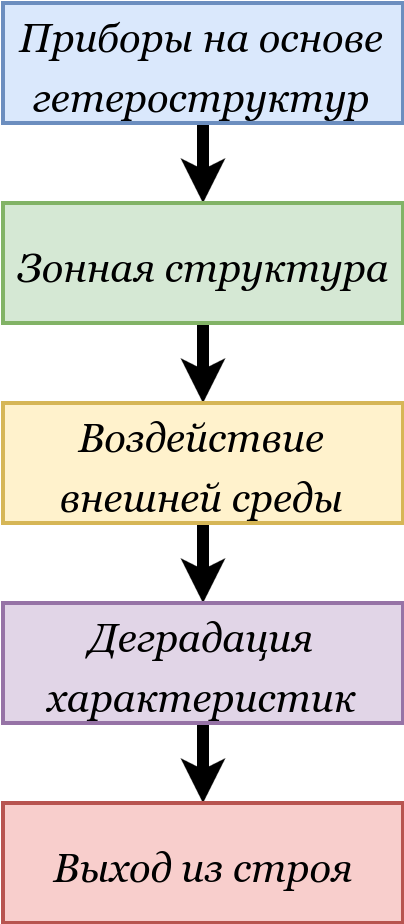
\includegraphics[width=\textwidth]{assets/Trouble}
		\end{center}
	\column{0.05\textwidth}
		\Huge{$\Rightarrow$}
	\column{0.33\textwidth}
		\begin{center}
			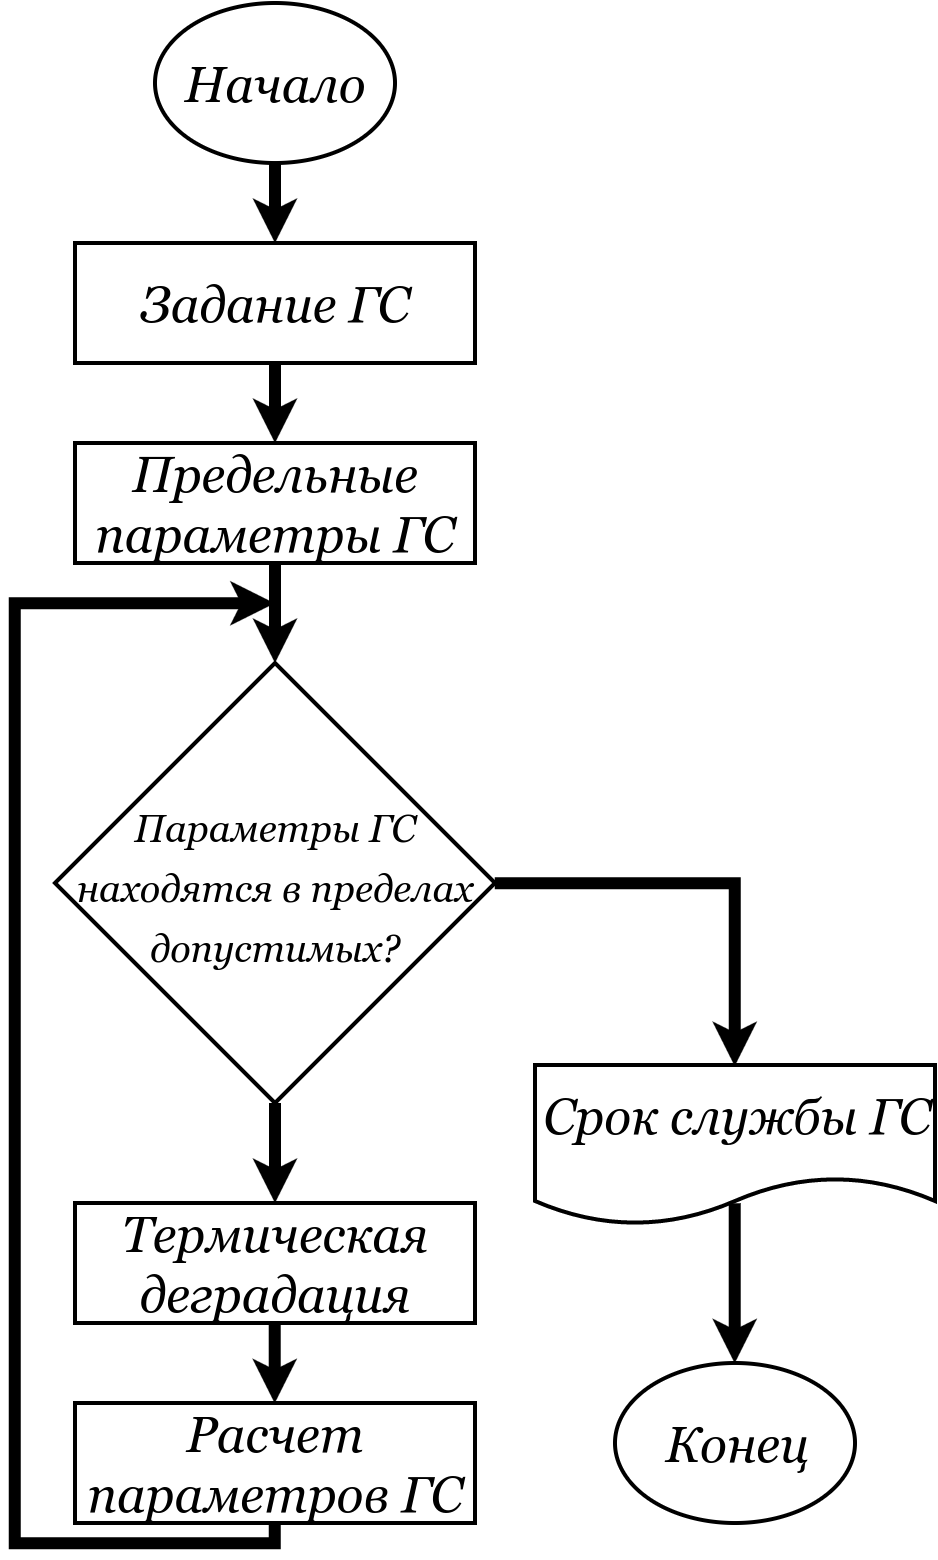
\includegraphics[width=\textwidth]{assets/AlgWrk}
		\end{center}
	\column{0.05\textwidth}
		\Huge{$\Rightarrow$}
	\column{0.33\textwidth}
		\begin{center}
			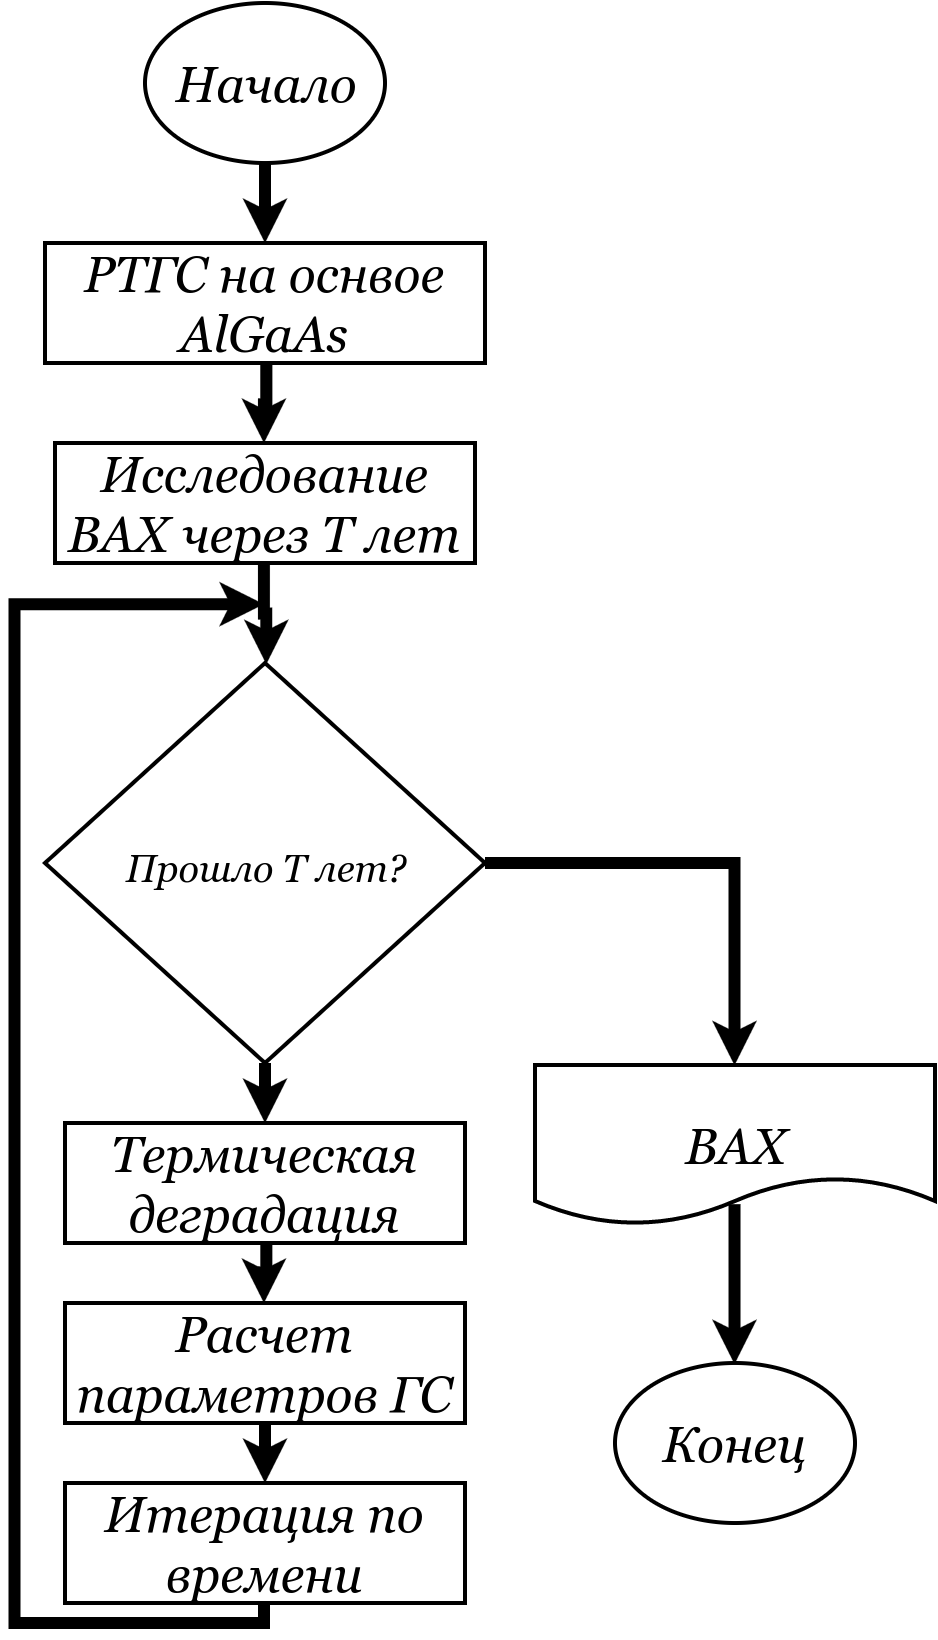
\includegraphics[width=0.95\textwidth]{assets/Cond}
		\end{center}
	\end{columns}
\end{frame}

\begin{frame}
	\frametitle{Цели и задачи}
	\color{blue}
	Цель работы:
	\begin{itemize}
		\item Разработка модели термической деградации слоистых гетероструктур на основе GaAs для интеграции в методику обеспечения заданного уровня надёжности устройства на их основе.
	\end{itemize}
	Задачи работы:
	\begin{itemize}
		\item Исследование математического аппарата для моделирования диффузионного размытия гетероструктур под действием градиента концентрации при фиксированной температуре системы;
		\item Исследование математического аппарата для моделирования токопереноса через гетероструктуру;
		\item Разработка алгоритма термической деградации гетероструктуры на основе $GaAs$.
	\end{itemize}
\end{frame}

\begin{frame}
	\frametitle{Численное моделирование физических процессов}
	\centering
	{\color{blue} Метод конечных разностей:}
	\begin{columns}
	\column{0.45\textwidth}
		\centering
			{\color{red}Аппроксимация первой производной:}
			\small
			\begin{gather*}
				\frac{d}{dx}S(x_{0}) = \frac{S(x_{0} + \Delta x) - S(x_{0})}{\Delta x };
			\end{gather*}
	\column{0.55\textwidth}
		\centering
		{\color{red}Аппроксимация второй производной:}
			\small
			\begin{gather*}
				\frac{d^{2}}{dx^{2}}S(x_{0})  = \frac{S(x_{0} + \Delta x) - 2S(x_{0}) + S(x_{0} - x \Delta)}{ \Delta x ^{2}};
			\end{gather*}
	\end{columns}
\rule{ \textwidth}{0.5mm}
{\color{blue} Конечно-разностная схема}
	\begin{columns}
	\column{0.4\textwidth}
		\centering
		{\color{red}Уравнения диффузии:}
		\begin{equation*}
			\frac{\delta}{\delta t} C = \frac{\delta}{\delta x}D\frac{\delta}{\delta x} C;
		\end{equation*}
	\column{0.6\textwidth}
		\centering
		{\color{red}Уравнение Шредингера:}
		\begin{equation*}
			-\frac{\hbar^{2}}{2}\frac{d}{dx}\frac{1}{m(x)}\frac{d}{dx}\psi(x) + U(x)\psi(x) = E\psi(x);
		\end{equation*}\\
	\end{columns}

	\begin{columns}
	\column{0.4\textwidth}
		\begin{center}
			\includegraphics[width=\textwidth]{assets/Diffusion}
		\end{center}
	\column{0.6\textwidth}
		\begin{center}
			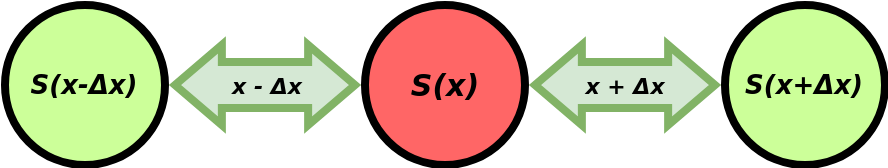
\includegraphics[width=.7\textwidth]{assets/Approx}
		\end{center}
	\end{columns}

\end{frame}

\begin{frame}
	\frametitle{Численное моделирование диффузии}
	{\color{blue}Коэффициент диффузии постоянен:}
	\begin{equation*}
		\begin{cases}
			D = Const;\\
			\frac{\delta}{\delta t} C = D \frac{\delta^{2}}{\delta x^{2}} C;
		\end{cases} \Rightarrow
		\frac{C^{i+1}_{j} - C^{i}_{j}}{\Delta t} = \frac{C^{i}_{j+1} - 2C^{i}_{j} + C^{i}_{j-1}}{\Delta x^2},\,\text{где }
		C^{i}_{j} = C(x_{j}, t_{i}).
	\end{equation*}

	\begin{columns}
	\column{0.5\textwidth}
		\centering
		{\color{red}<<Закрытая>> система:}\\
		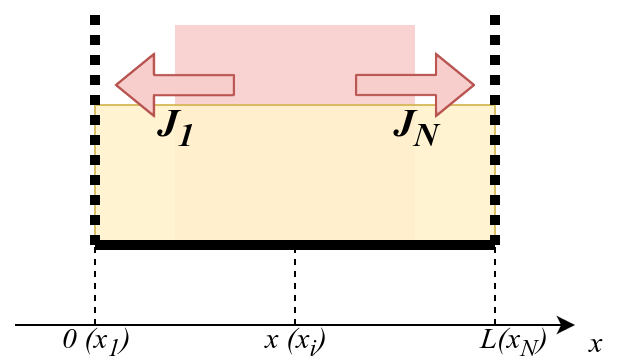
\includegraphics[width=0.77\linewidth]{assets/CD}
		\small
		\begin{equation*}
		\begin{cases}
			C^{i+1}_{1} = (1 - \lambda)C^{i}_{1} + \lambda C^{i}_{2};\\
			C^{i+1}_{j} = \lambda C^{i}_{j-1} + (1 - 2\lambda)C^{i}_{j} + \lambda C^{i}_{j+1};\\
			C^{i+1}_{N} = (1 - \lambda)C^{i}_{N} + \lambda C^{i}_{N-1};\\
			\lambda = D\frac{\Delta t}{\Delta x^{2}}.
		\end{cases}
		\end{equation*}
	\column{0.5\textwidth}
		\centering
		{\color{red}<<Открытая>> система:}\\
	   	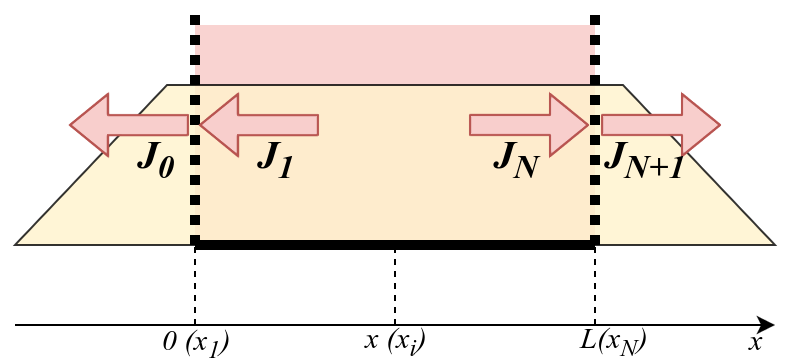
\includegraphics[width=\linewidth]{assets/OD}
		\small
		\begin{equation*}
		\begin{cases}
			C^{i+1}_{1} = C^{i}_{1};\\
			C^{i+1}_{j} = \lambda C^{i}_{j-1} + (1 - 2\lambda)C^{i}_{j} + \lambda C^{i}_{j+1};\\
			C^{i+1}_{N} = C^{i}_{N};\\
			\lambda = D\frac{\Delta t}{\Delta x^{2}}.
		\end{cases}
		\end{equation*}
	\end{columns}
\end{frame}

\begin{frame}
	\frametitle{Численное моделирование диффузии}
Диффузионное размытие {\color{blue} $i$-$GaAs/i$-$Al_{x}Ga_{1-x}As/i$-$GaAs$}:
	\begin{columns}
	\column{0.7\textwidth}
		\begin{equation*}
			\label{eq:DNd}
			D_{Al} = D_{0}\exp\bigg[-\frac{E_{a}}{k_{B}T}\bigg] = D_{0}\exp\bigg[-\frac{3.5}{k_{B}T}\bigg]
		\end{equation*}
	\column{0.3\textwidth}
		\begin{itemize}
			\item $a = 10$ нм;
			\item $b = 30$ нм;
		\end{itemize}
	\end{columns}

	\begin{columns}
	\column{0.5\textwidth}
	\centering
		{\color{red}<<Закрытая>> система:}\\
	   	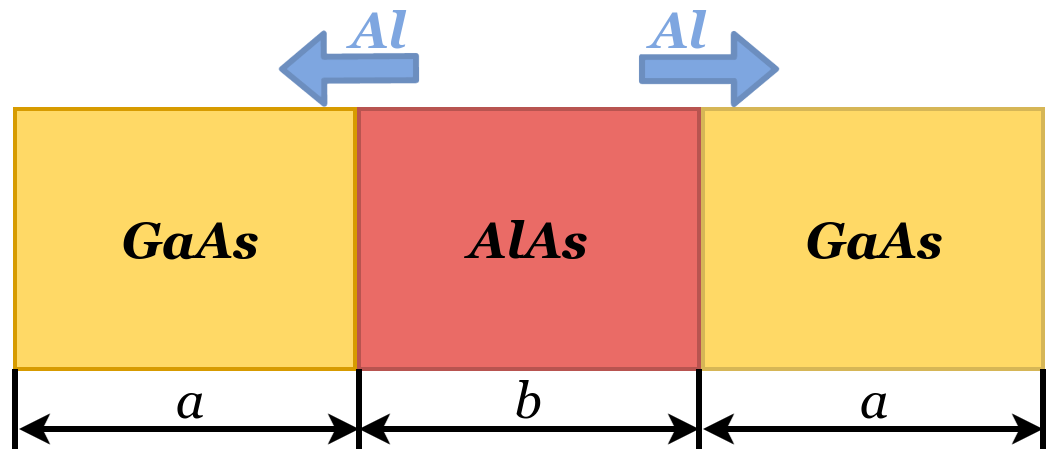
\includegraphics[width=0.6\linewidth]{assets/DCloseBox}\\
	   	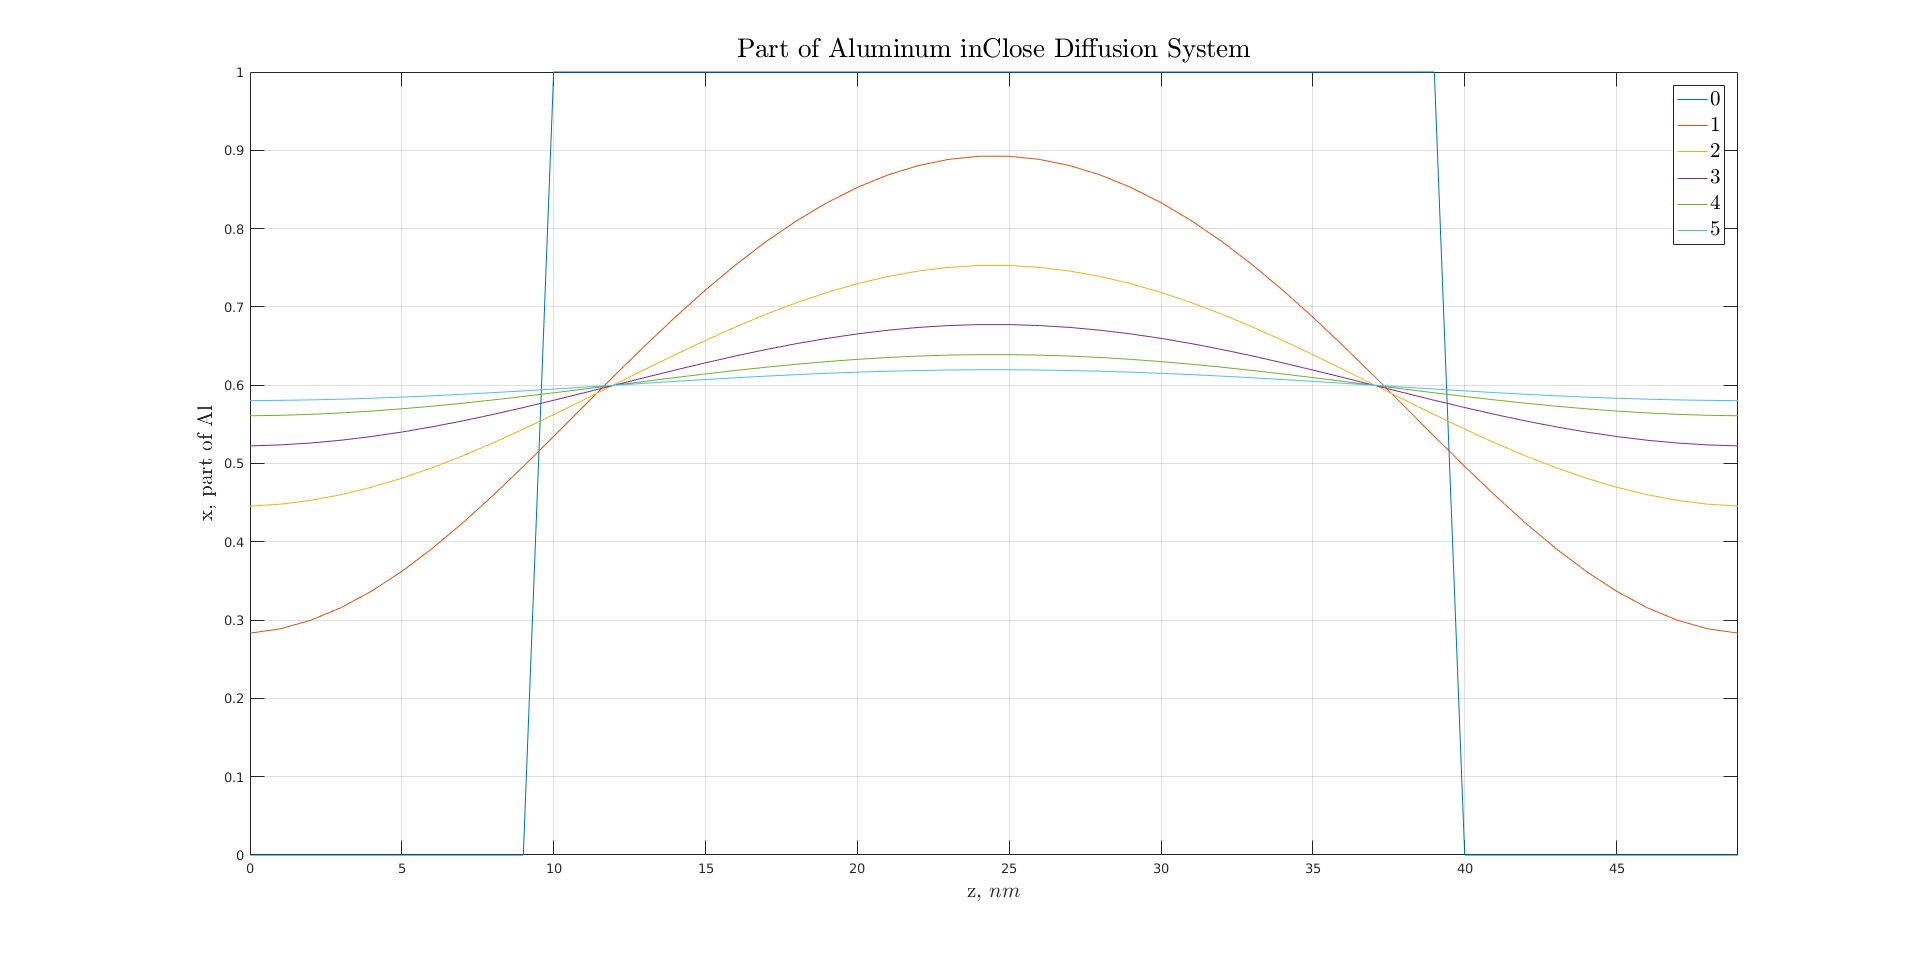
\includegraphics[width=\linewidth]{assets/DCAl}
	\column{0.5\textwidth}
	\centering
		{\color{red}<<Открытая>> система:}\\
	   	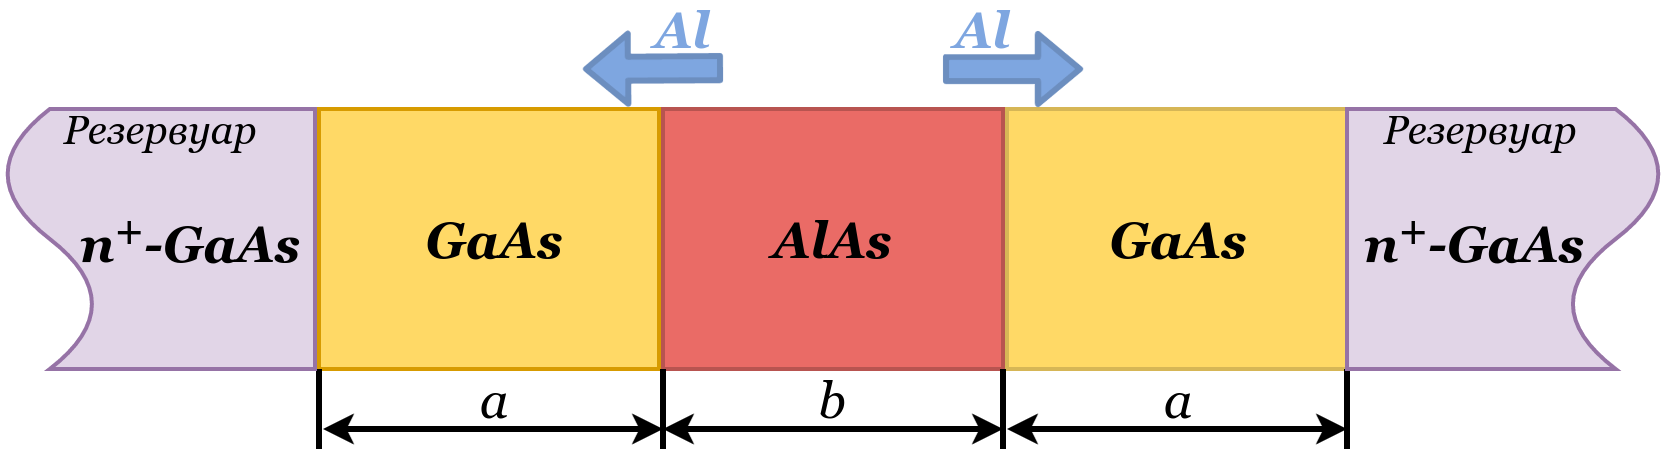
\includegraphics[width=\linewidth]{assets/DOpenBox}\\
	   	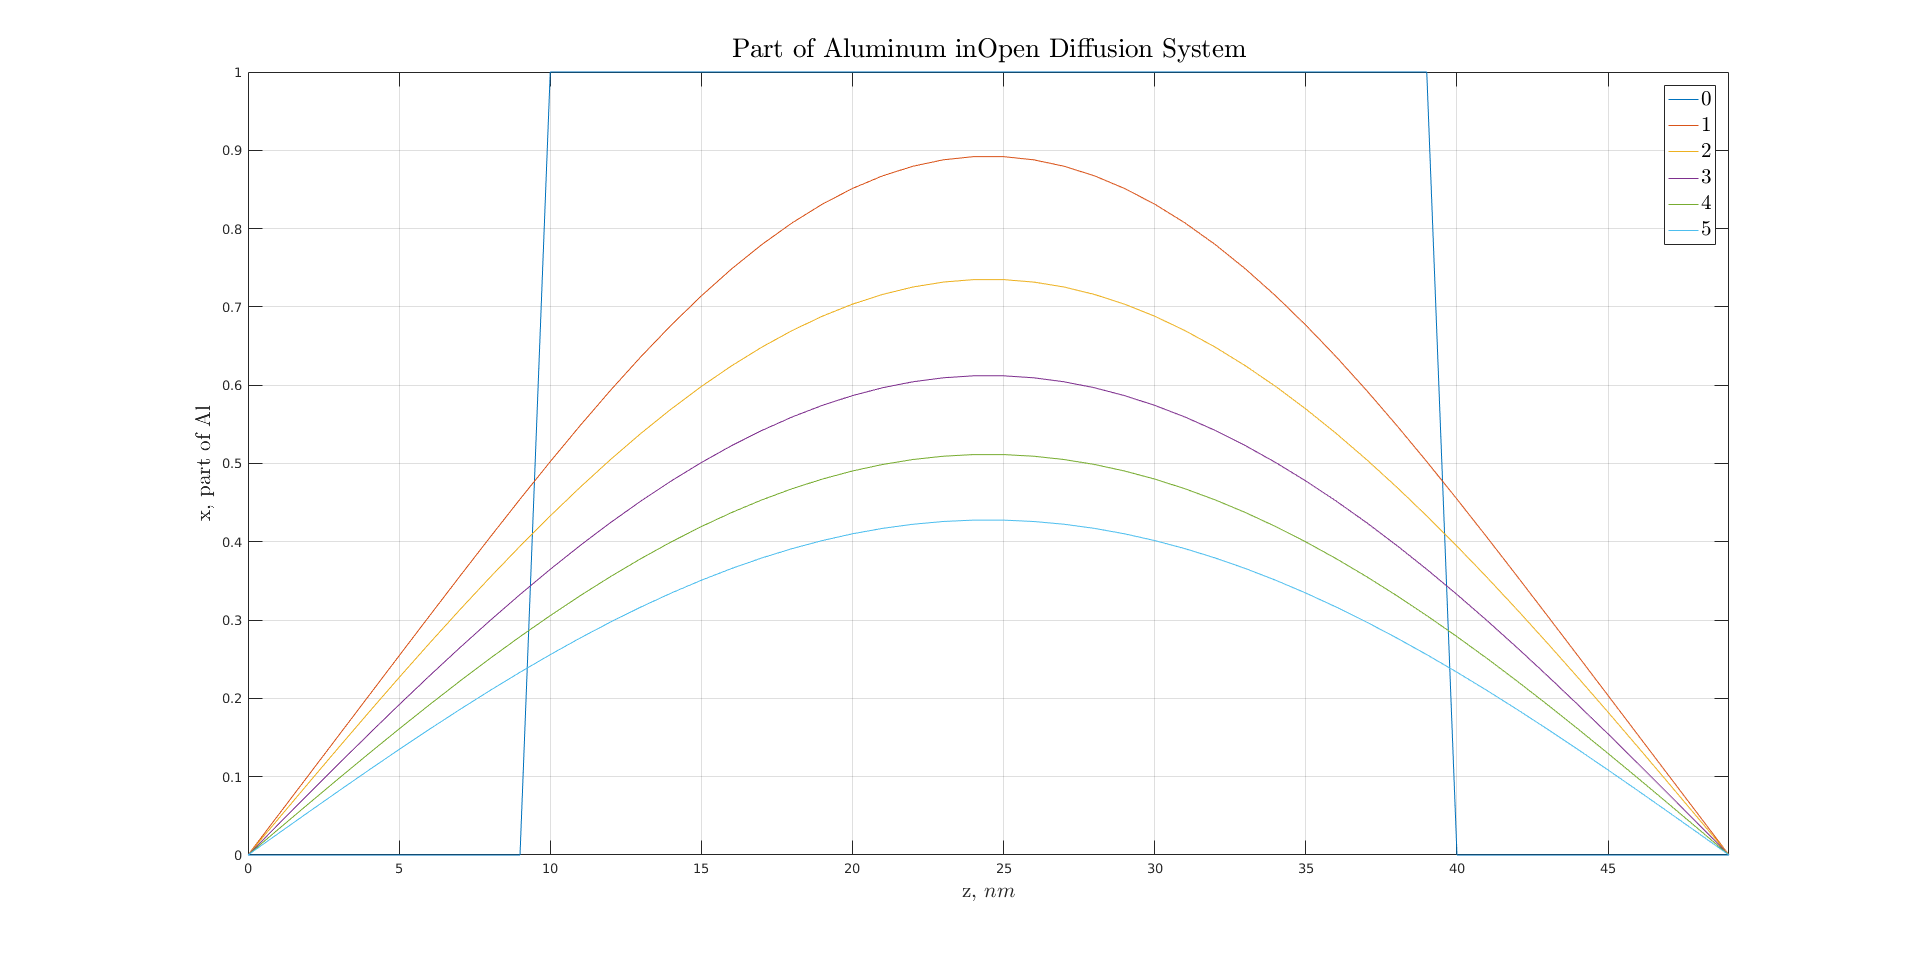
\includegraphics[width=\linewidth]{assets/DOAl}

	\end{columns}
\end{frame}

\begin{frame}
	\frametitle{Численное моделирование диффузии}
	{\color{blue}Коэффициент диффузии зависит от концентрации}:
	\small
	\begin{equation*}
		\begin{cases}
			D \neq Const;\\
			\frac{\delta}{\delta t} C = \frac{\delta}{\delta x} D \frac{\delta}{\delta x} C;
		\end{cases} \Rightarrow
		\frac{C_{j}^{i+1} - C_{j}^{i}}{\Delta t} = \frac{ D_{j+1/2}^{i}\frac{C^{i}_{j+1} - C^{i}_{j}}{\Delta x} - D_{j-1/2}^{i}\frac{C^{i}_{j} - C^{i}_{j-1}}{\Delta x} }{\Delta x},\,\text{где }		
		\begin{cases}
			D_{j\pm1/2}^{i} = \frac{D^{i}_{j} + D^{i}_{j\pm1}}{2} = D_{j\pm}^{i};\\
			C^{i}_{j} = C(x_{j}, t_{i}).
		\end{cases}
	\end{equation*}
		{\color{red}<<Открытая>> система с проникновением примеси из границ исследуемой области:}\\
		\begin{columns}
		\column{0.45\textwidth}
		   	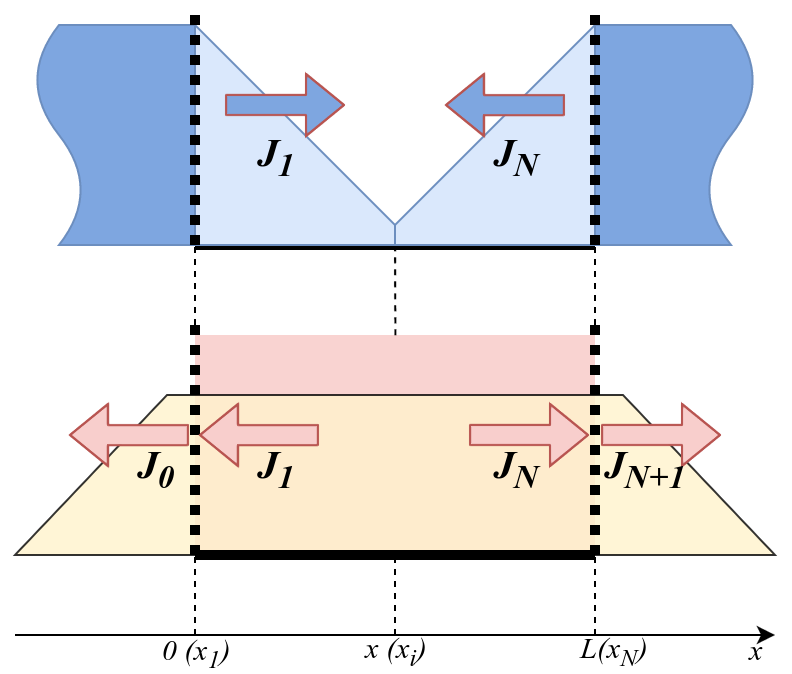
\includegraphics[width=\linewidth]{assets/ODSI}
		\column{0.55\textwidth}
			\large
			\begin{equation*}
				\label{eq:DFromC}
				\begin{cases}
					C^{i+1}_{1} = C^{i}_{1};\\
					C^{i+1}_{j} = \lambda_{-}^{i} C^{i}_{j-1} + (1 - \lambda^{i}_{+} - \lambda^{i}_{-})C^{i}_{j} + \lambda^{i}_{+} C^{i}_{j+1};\\
					C^{i+1}_{N} = C^{i}_{N};\\
					\lambda^{i}_{+} = D_{j+}^{i}\frac{\Delta t}{\Delta x^{2}};\\
					\lambda^{i}_{-} = D_{j-}^{i}\frac{\Delta t}{\Delta x^{2}}.
				\end{cases}
			\end{equation*}
		\end{columns}

\end{frame}
\begin{frame}
	\frametitle{Численное моделирование диффузии}
	Диффузионное размытие {\color{blue} $n^{+}$-$GaAs/i$-$GaAs/i$-$Al_{x}Ga_{1-x}As/i$-$GaAs/n^{+}$-$GaAs$}:
	\begin{equation*}
		D_{Al,Si} = D_{0}\exp\bigg[-\frac{E_{a}}{k_{B}T}\bigg]\Big( \frac{N_{D}}{n_{i}} \Big)^{3} = D_{0}\exp\bigg[-\frac{3.5}{k_{B}T}\bigg]\Big( \frac{N_{D}}{n_{i}} \Big)^{3}
	\end{equation*}
	{\color{red}<<Открытая>> система с проникновением частиц из границ исследуемой области:}\\
	\centering
   	% 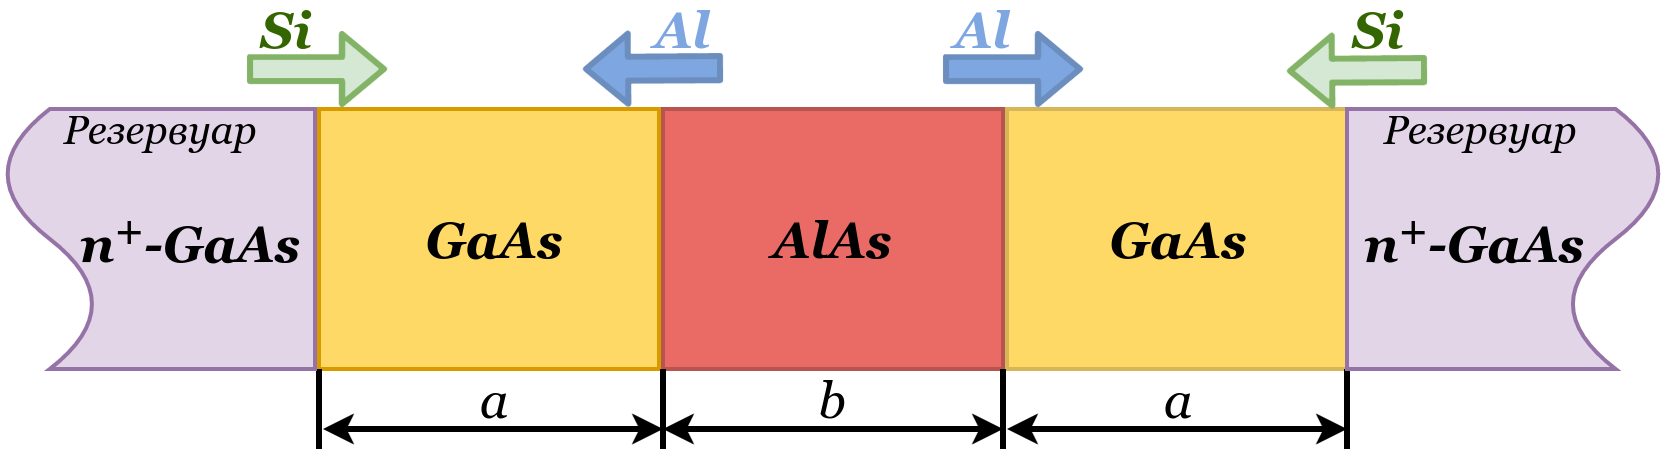
\includegraphics[width=0.3\linewidth]{assets/DSiBox}\\
   	% 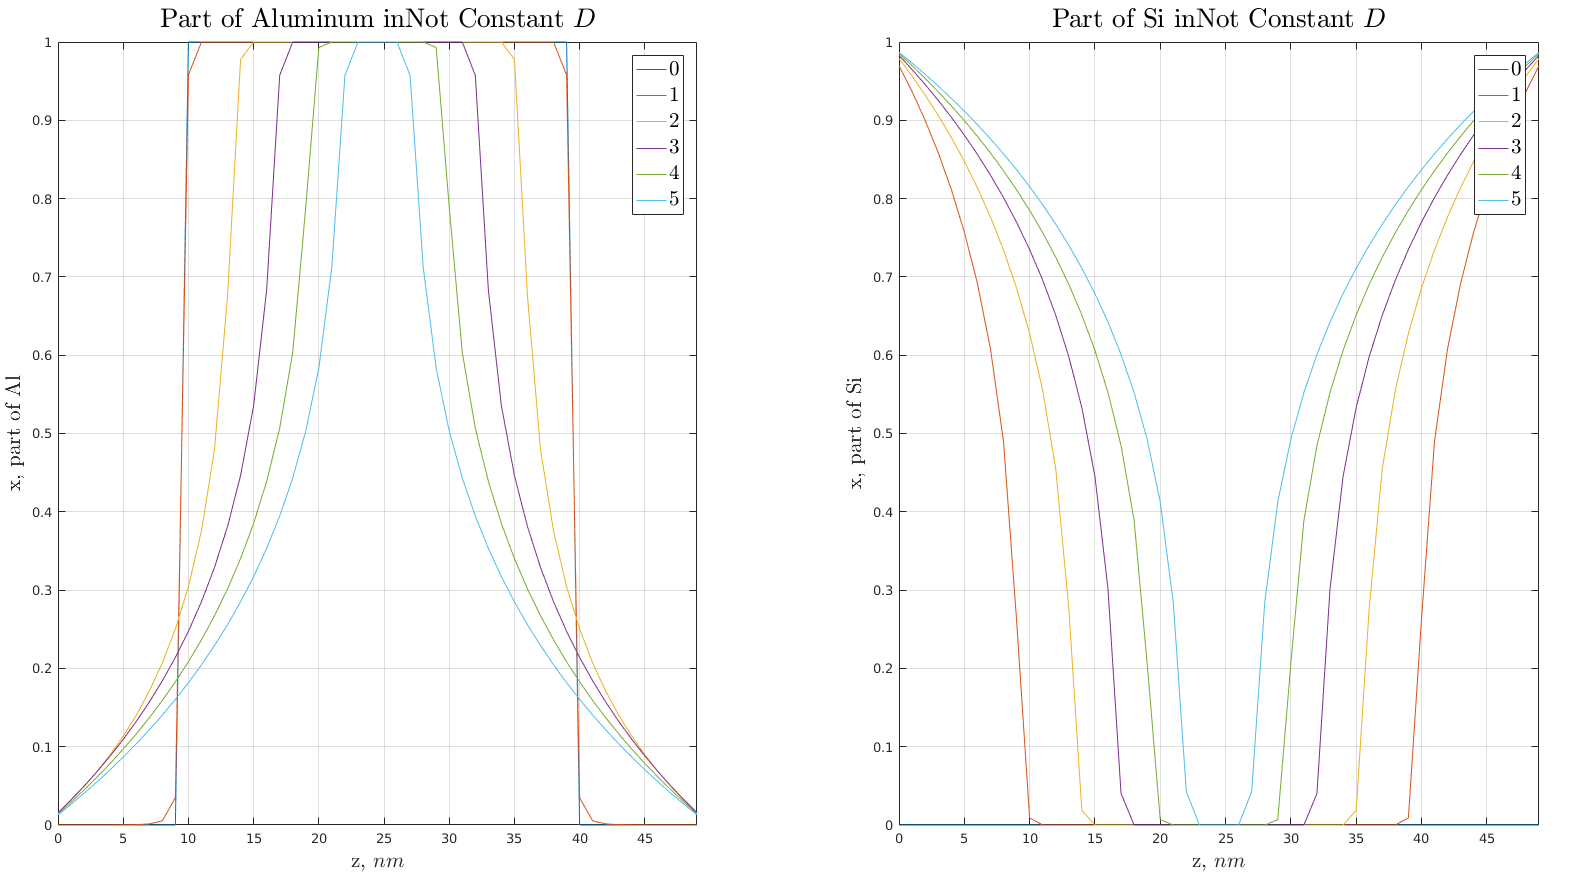
\includegraphics[width=0.6\linewidth]{assets/DSi}
\begin{columns}
\column{0.4\textwidth}
   	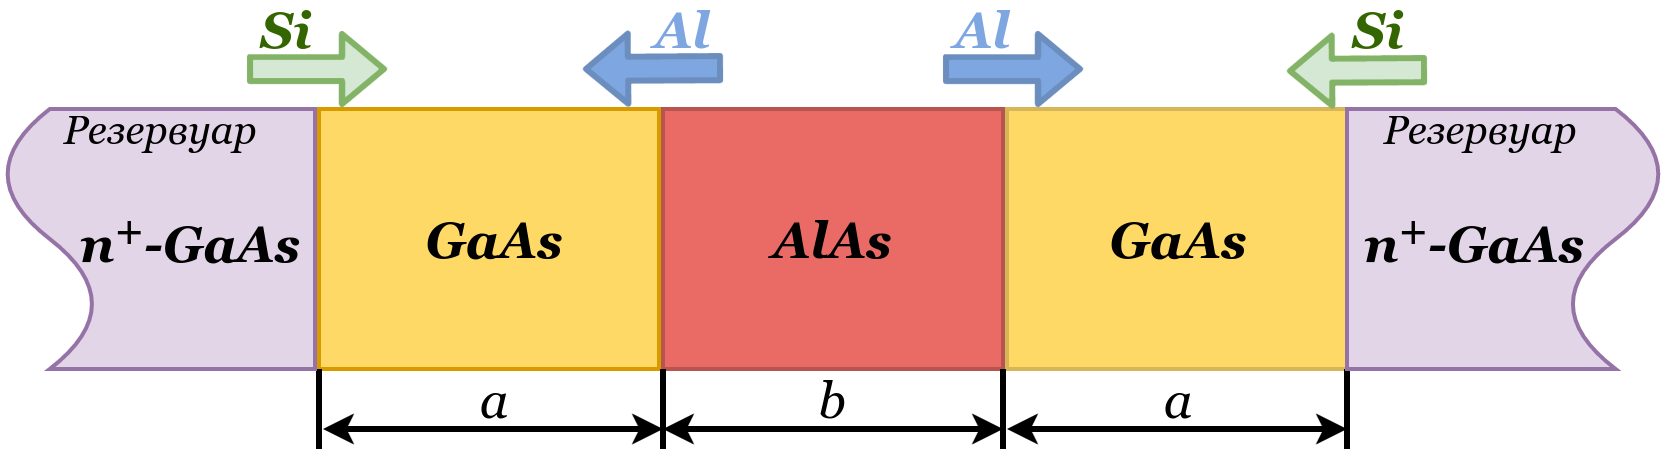
\includegraphics[width=\linewidth]{assets/DSiBox}
   	\begin{itemize}
   		\item $a = 10$ нм;
   		\item $b = 30$ нм;
   	\end{itemize}
\column{0.6\textwidth}
   	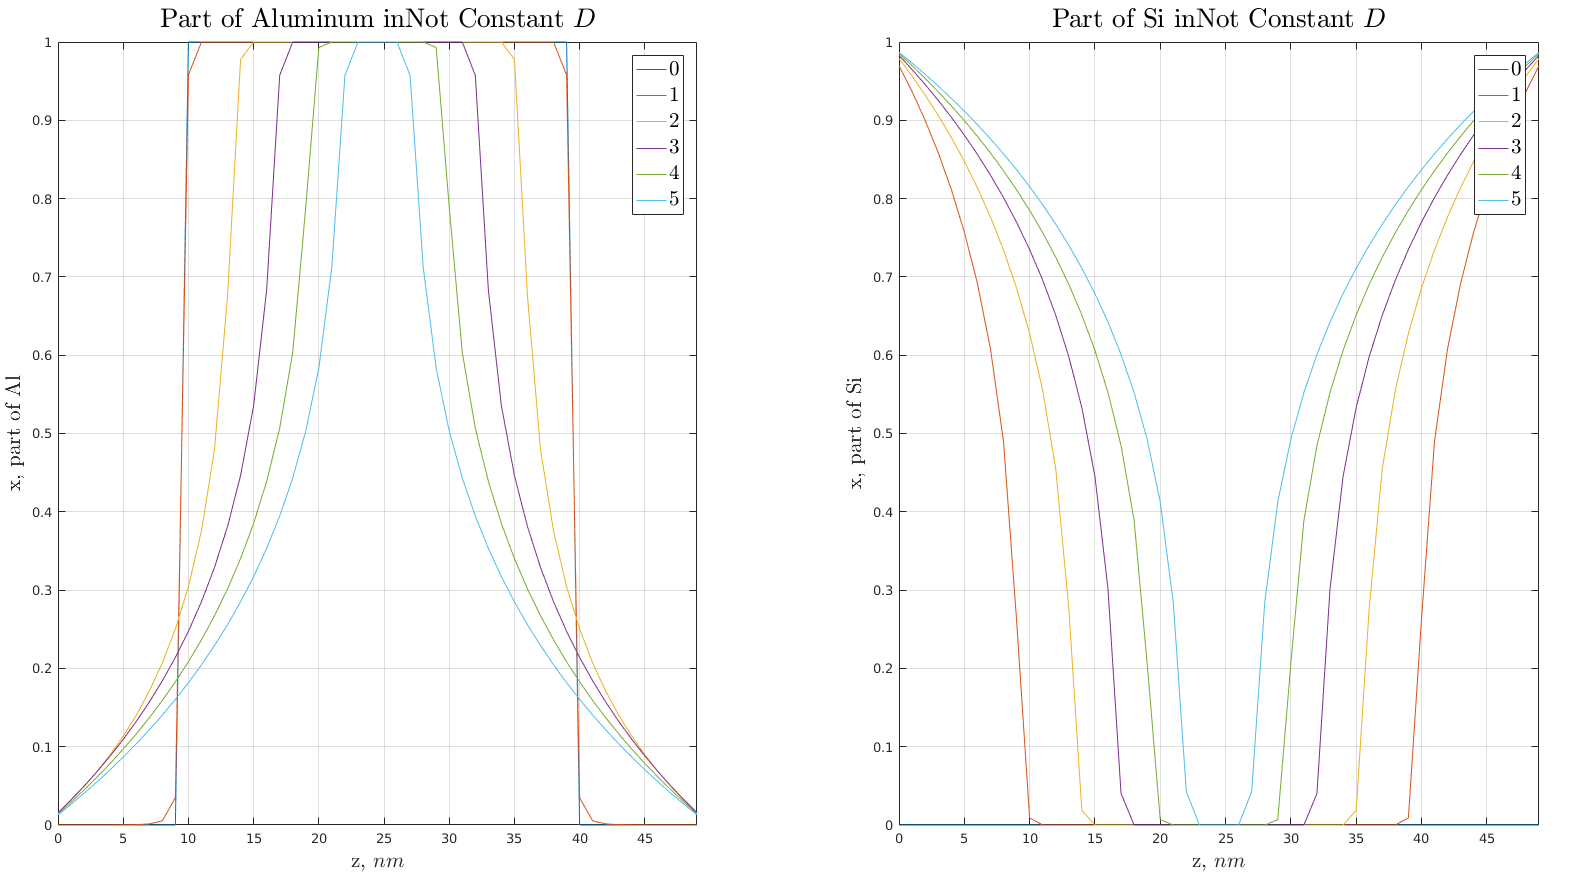
\includegraphics[width=\linewidth]{assets/DSi}
\end{columns}
\end{frame}

\begin{frame}
	\frametitle{Численное моделирование токопереноса}

\begin{columns}
\column{0.275\textwidth}
	\centering
	{\color{blue}\large Формула Цу-Есаки:}
\column{0.72\textwidth}
	\centering
	{\color{blue}\large Численное решение уравнение Шредингера:}
\end{columns}


\begin{columns}
\column{0.29\textwidth}
	% {\color{blue}\large Формула Цу-Есаки:}
	{\footnotesize
	\begin{gather*}
		J(V) = \frac{2mek_{B}T}{(2\pi)^{2}\hbar^{3}}\int\limits_{0}^{\infty}T(E)D(E)dE;
	\end{gather*}}
	{\color{red}Функция снабжения:}
	{\footnotesize
	\begin{gather*}
		D(E) = \ln\frac{1 + \exp{\frac{E_{F}-E}{k_{B}T}} }{ 1 + \exp{\frac{E_{F}-E-eV}{k_{B}T}} };
	\end{gather*}}
	{\color{red}Прозрачность ГС:}
	{\footnotesize
	\begin{gather*}
		T(E) = |T_{L}|^{2}\frac{|k_{R}|m_{L}}{|k_{L}|m_{R}};\\
		\psi_{L} = \exp [ik_{L}z];\\
		\psi_{R} = T_{L}\psi_{L} = T_{L}\exp [ik_{L}z];
	\end{gather*}}
\column{0.01\textwidth}
	\rule[1mm]{0.2ex}{70mm}
\column{0.72\textwidth}
	% {\color{blue}\large Численное решение уравнение Шредингера:}
   	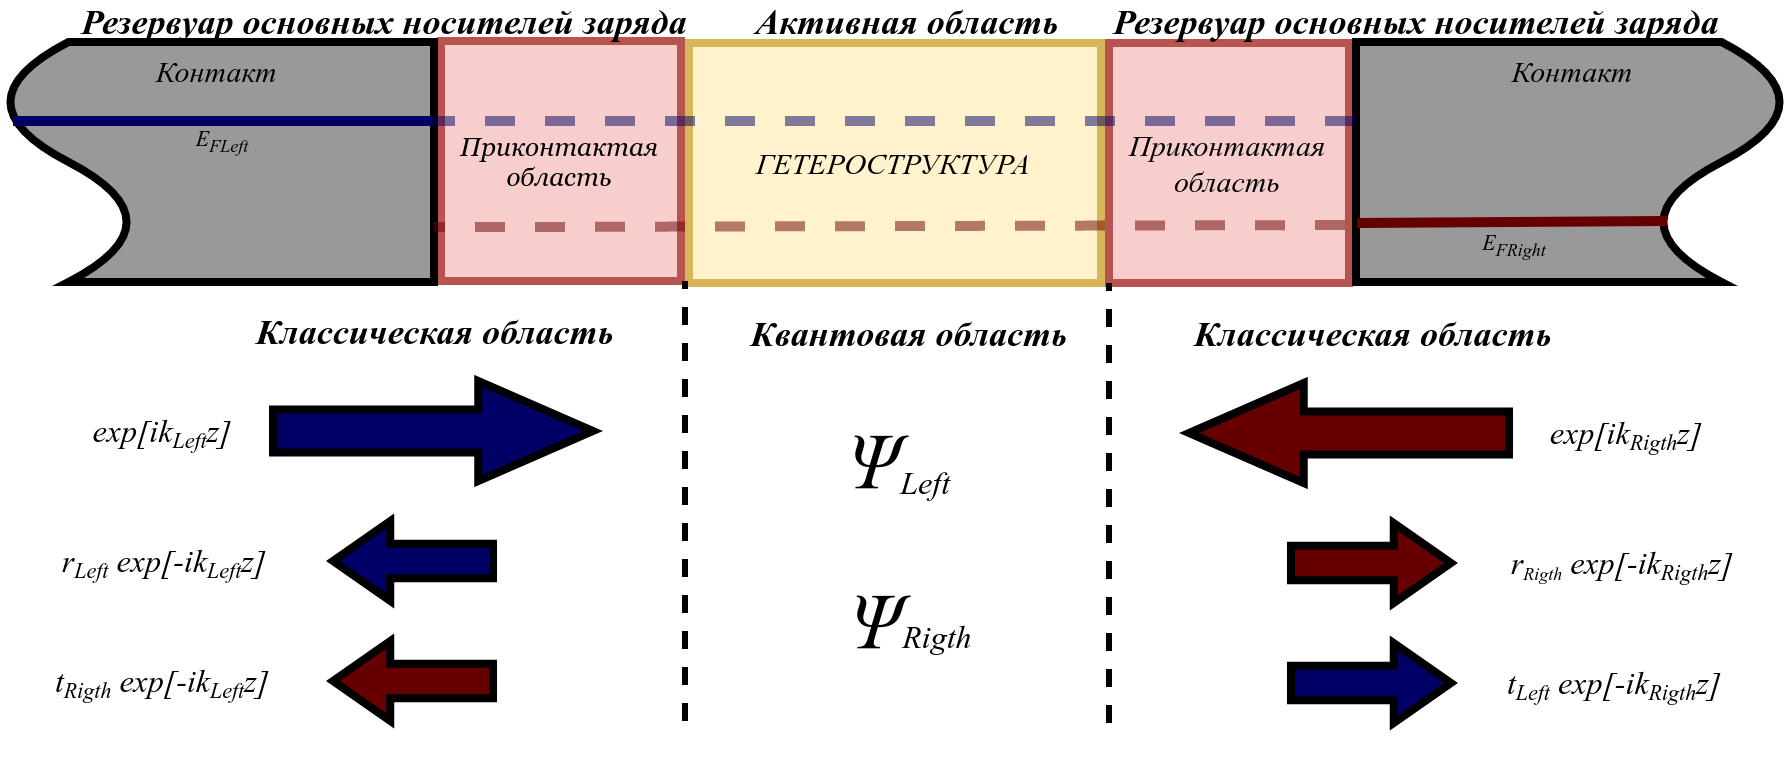
\includegraphics[width=\linewidth]{assets/HSModel}

   	{\color{red}Конечно-разностная схема для внутренних точек:}
   	
   	{\scriptsize
	\begin{equation*}
		\psi_{i-1}\frac{m^{*}_{i+1}}{m^{*}_{i-1}} + \psi_{i}\bigg(  \frac{2\Delta^{2}m^{*}_{i+1}}{\hbar^{2}}(E-U_{i}) - \frac{m^{*}_{i+1}}{m^{*}_{i-1}} - 1 \bigg) + \psi_{i+1} = 0,
	\end{equation*}}


{\color{red}Конечно-разностная схема для граничных точек:}
\begin{columns}
\column{0.5\textwidth}
	\footnotesize
	\begin{gather*}
		\begin{cases}
			(ik_{L}-1)\psi_{1} + \psi_{2} = 2ik_{L}\Delta;\\
			\psi_{N-1} + (ik_{R}\Delta - 1)\psi_{N} = 0;
		\end{cases}
	\end{gather*}
\column{0.5\textwidth}
	\footnotesize
	\begin{gather*}
		\begin{cases}
			(ik_{L}-1)\psi_{1} + \psi_{2} = 0\Delta;\\
			\psi_{N-1} + (ik_{R}\Delta - 1)\psi_{N} = 2ik_{R}\Delta;;
		\end{cases}
	\end{gather*}
\end{columns}
\end{columns}
\end{frame}

\begin{frame}
	\frametitle{Численное моделирование токопереноса}
	\begin{columns}
	\column{0.5\textwidth}
	   	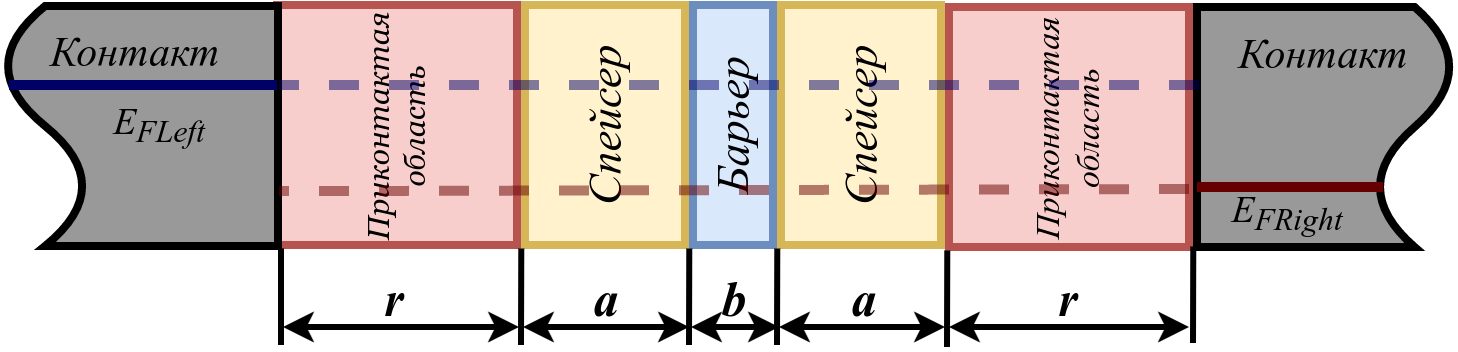
\includegraphics[width=\linewidth]{assets/BHS}

		{\scriptsize $\bullet$ $a = 5$ нм; $\bullet$ $b = 5$ нм; $\bullet$ $\Delta E_{c} = 1$эВ.}
	\column{0.01\textwidth}
		\rule[1mm]{0.2ex}{70mm}
	\column{0.5\textwidth}
	   	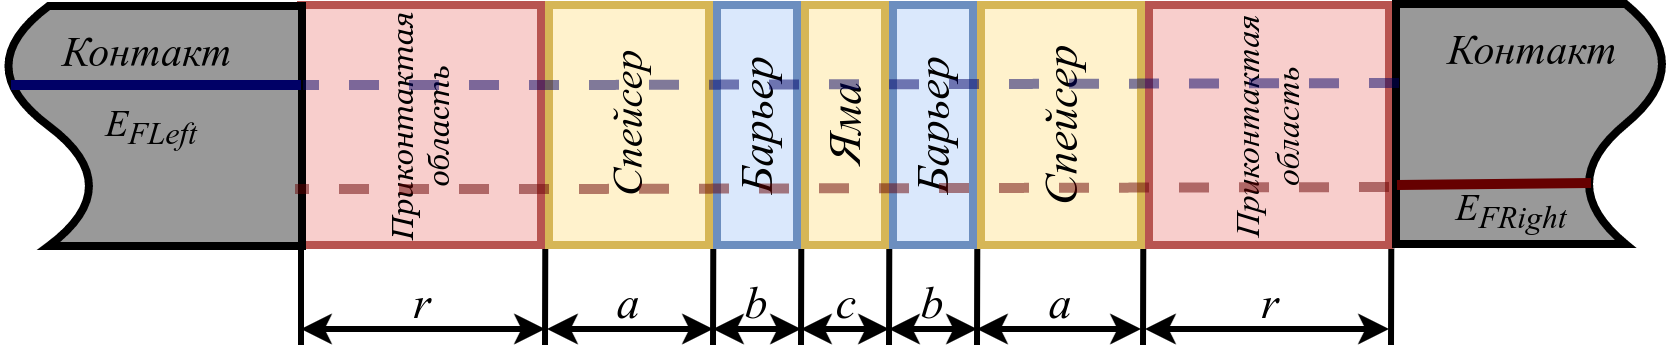
\includegraphics[width=\linewidth]{assets/RTHS}

		{\scriptsize $\bullet$ $a = 5$ нм; $\bullet$ $b = 5$ нм; $\bullet$ $c = 5$ нм; $\bullet$ $\Delta E_{c} = 1$эВ.}
	\end{columns}
\end{frame}

\begin{frame}
	\frametitle{Учет самосогласованного потенциала}
	{\color{blue}Уравнеие Пуассона:}
	\begin{equation*}
		\frac{d}{dz}\varepsilon(z)\frac{d}{z}V_{s} = \frac{e}{\varepsilon_{0}}[n(z) - N_{D}(z)];
	\end{equation*}

\begin{columns}
\column{0.5\textwidth}
	{\color{red}Концентрация электронов в ГС:}
	\footnotesize
	\begin{gather*}
		{\tiny \begin{cases}
					\sum\limits_{L,R}\int\limits_{U_{l(r)}}^{\infty} \frac{|\psi_{L(R)}|^{2}}{\sqrt{E - U_{L(R)}}} \ln \bigg( 1 + \exp\bigg[ -\frac{E - E_{F} - U_{la(ra)}}{k_{B}T} \bigg] \bigg);\\
					N^{3D} \int\limits_{0}^{+\infty}\! \frac{\sqrt[]{E}}{e^{\frac{E-\mu}{kT}}+1} \,dE;
				\end{cases}}\\
		N^{A} = \frac{2^{1/2}m^{3/2}k_{B}T}{(2\pi)^{2}\hbar^{3}};\\
		N^{3D} = \frac{2^{1/2}m^{3/2}}{\pi^{2}\hbar^{3}}; 
	\end{gather*}
\column{0.5\textwidth}
	{\color{red}Конечно-разностная схема. Метод Гулеля:}
	\tiny
	\begin{gather*}
	n(z) = n_{0}\exp\frac{V_{S}(z)}{V_{ref}};\,
	n_{0} = \frac{2^{1/2}m^{3/2}k_{B}T}{(2\pi)^{2}\hbar^{3}} \exp \frac{E_{F} - E_{c} }{k_{B}T};\,
	V_{ref} = \frac{k_{B}T}{e};\\
	n_{new} = n_{old}\exp\frac{V_{new} - V_{old}}{V_{ref}}
\end{gather*}
\begin{equation*}
	\frac{d}{dz}\varepsilon(z)\frac{d}{z}V_{new} - n_{old}\frac{eV_{new}}{\varepsilon_{0}V_{ref}} = \frac{e}{\varepsilon_{0}}\bigg[n_{old}\bigg( 1 - \frac{V_{old}}{V_{ref}} \bigg) - N_{D}(z)\bigg];
\end{equation*}
\end{columns}
\end{frame}

\begin{frame}
	\frametitle{Исследование влияния параметров РТГС на ВАХ}
	{\color{blue} Исследуемая модель:}
	\begin{columns}
	\column{0.35\textwidth}
	   	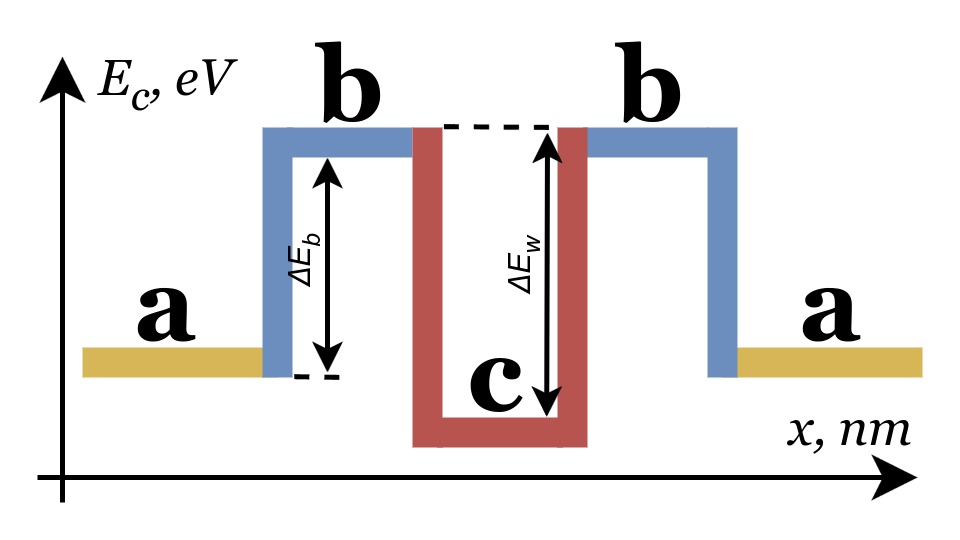
\includegraphics[width=\linewidth]{assets/BD}
	\column{0.65\textwidth}
	   	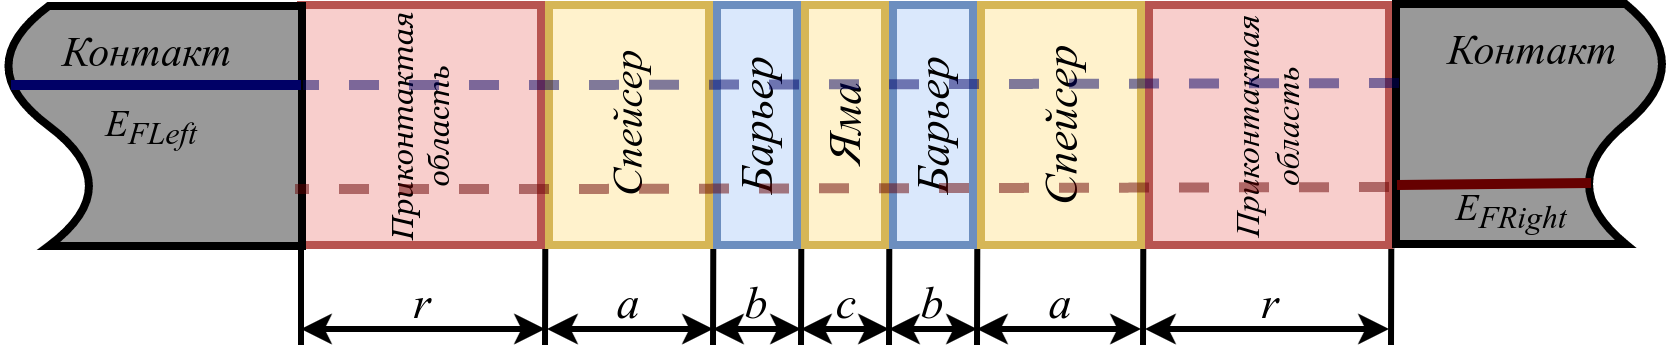
\includegraphics[width=\linewidth]{assets/RTHS}
	\end{columns}

\begin{columns}
\column{0.33\textwidth}
	{\color{red} Параметры ямы:}
	\footnotesize
	\begin{itemize}
		\item Ширина ямы (<<c>>): \begin{itemize}
			\footnotesize
			\item 10 монослоев;
			\item 7 монослоев;
			\item 5 монослоев;
			\item 3 монослоев;
		\end{itemize}
		\item Глубина ямы (<<$\Delta E_{w}$>>): \begin{itemize}
			\footnotesize
			\item 0.3 eV;
			\item 0.7 eV;
			\item 1 eV;
			\item 1.3 eV;
		\end{itemize} 
	\end{itemize}
\column{0.01\textwidth}
	\rule[0mm]{0.2ex}{40mm}
\column{0.33\textwidth}
	{\color{red} Параметры барьеров:}
	\footnotesize
	\begin{itemize}
		\item Ширина барьеров (<<b>>): \begin{itemize}
			\footnotesize
			\item 10 монослоев;
			\item 7 монослоев;
			\item 5 монослоев;
			\item 3 монослоев;
		\end{itemize}
		\item Высота барьера (<<$\Delta E_{b}$>>): \begin{itemize}
			\footnotesize
			\item 0.3 eV;
			\item 0.5 eV;
			\item 0.7 eV;
			\item 1 eV;
		\end{itemize} 
	\end{itemize}
\column{0.01\textwidth}
	\rule[0mm]{0.2ex}{40mm}
\column{0.33\textwidth}
	{\color{red} Параметры спейсеров:}
	\footnotesize
	\begin{itemize}
		\item Ширина спейсера (<<a>>): \begin{itemize}
			\footnotesize
			\item 10 монослоев;
			\item 7 монослоев;
			\item 5 монослоев;
			\item 3 монослоев;
		\end{itemize}
		\item Ширина спейсера с ССП: \begin{itemize}
			\footnotesize
			\item 10 монослоев;
			\item 7 монослоев;
			\item 5 монослоев;
			\item 3 монослоев;
		\end{itemize} 
	\end{itemize}
\end{columns}
\end{frame}

\begin{frame}
	\frametitle{Исследование влияния параметров ямы РТГС на ВАХ}
	\begin{columns}
	\column{0.5\textwidth}
		{\color{blue} Ширина ямы:}\\
		{\color{red} Прозрачность РТГС:}
	   	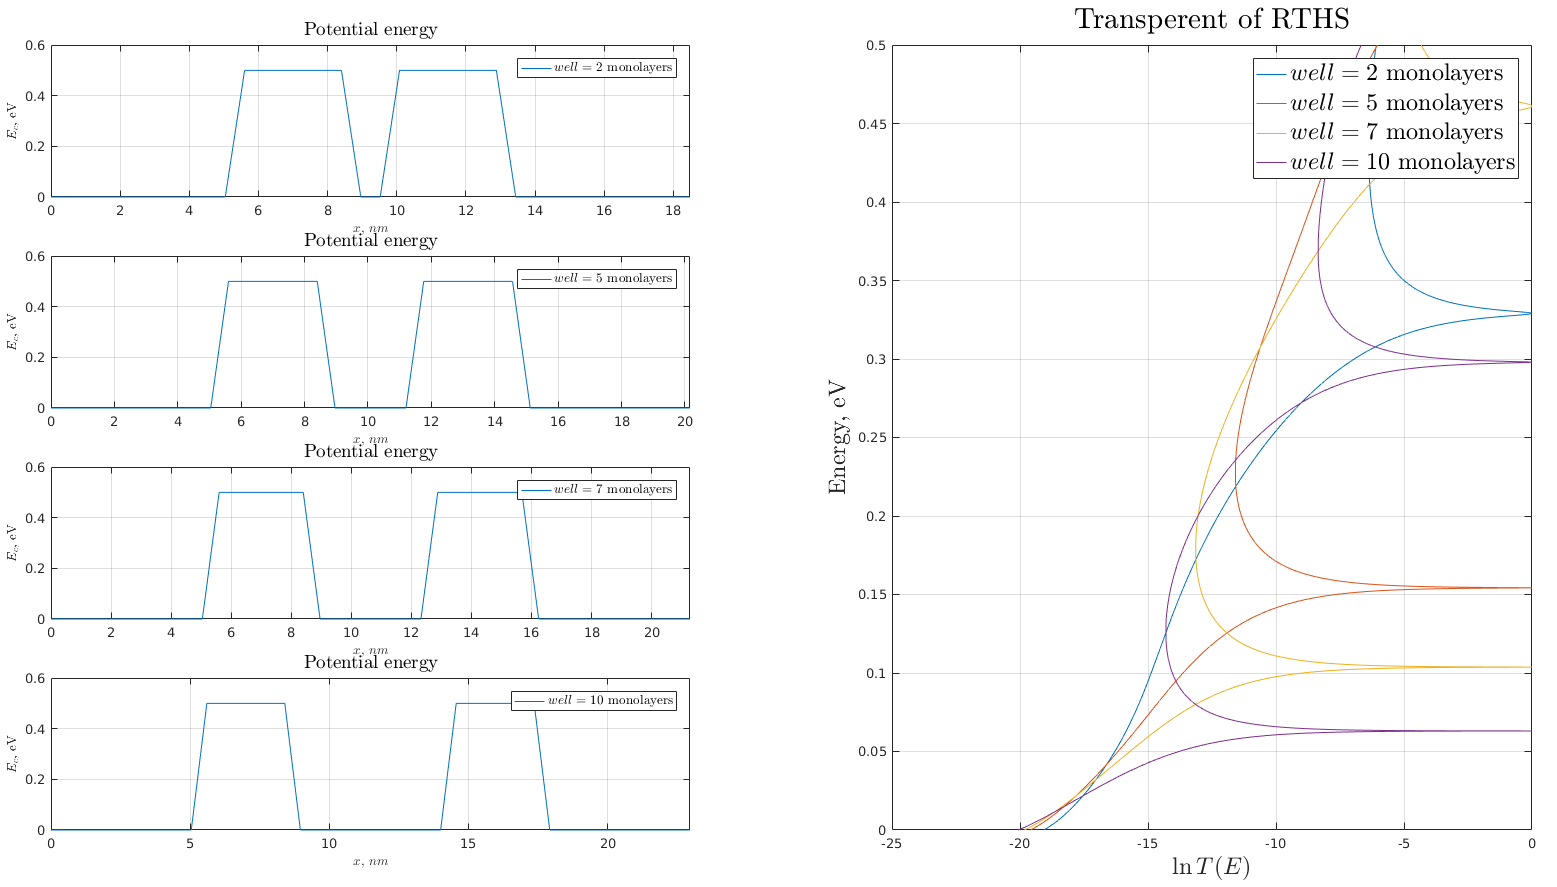
\includegraphics[width=.88\linewidth,center]{assets/qwwt}\\
		{\color{red} Плотность тока через РТГС:}
	   	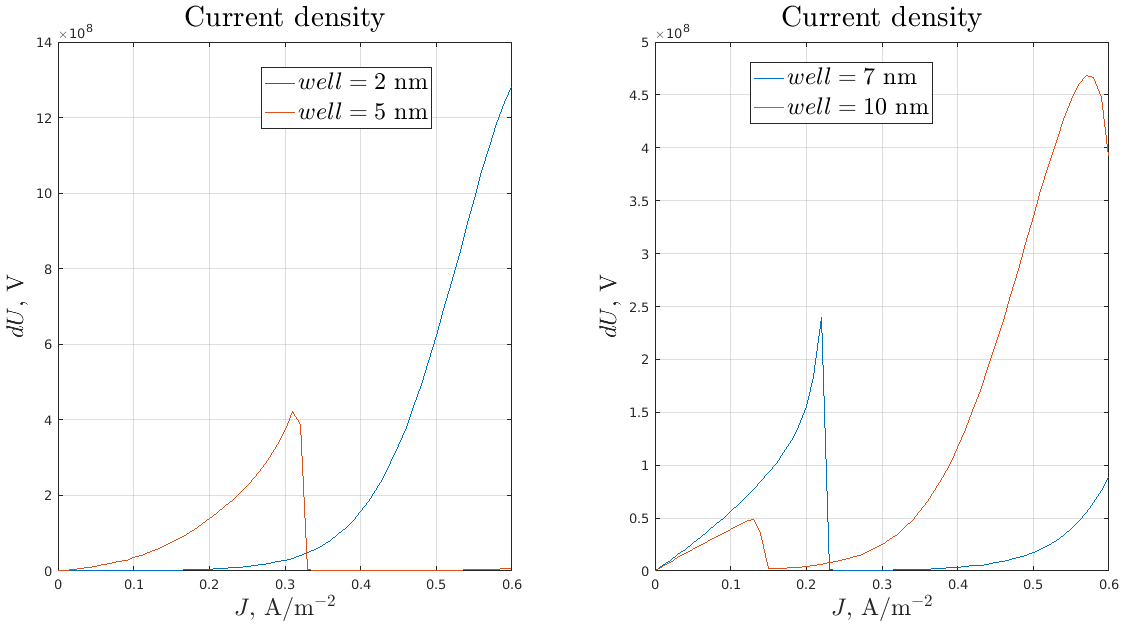
\includegraphics[width=.88\linewidth,center]{assets/qwwj}
	\column{0.01\textwidth}
		\rule[-55mm]{0.2ex}{75mm}
	\column{0.5\textwidth}
		{\color{blue} Глубина ямы:}\\
		{\color{red}\small Прозрачность РТГС:}\\
	   	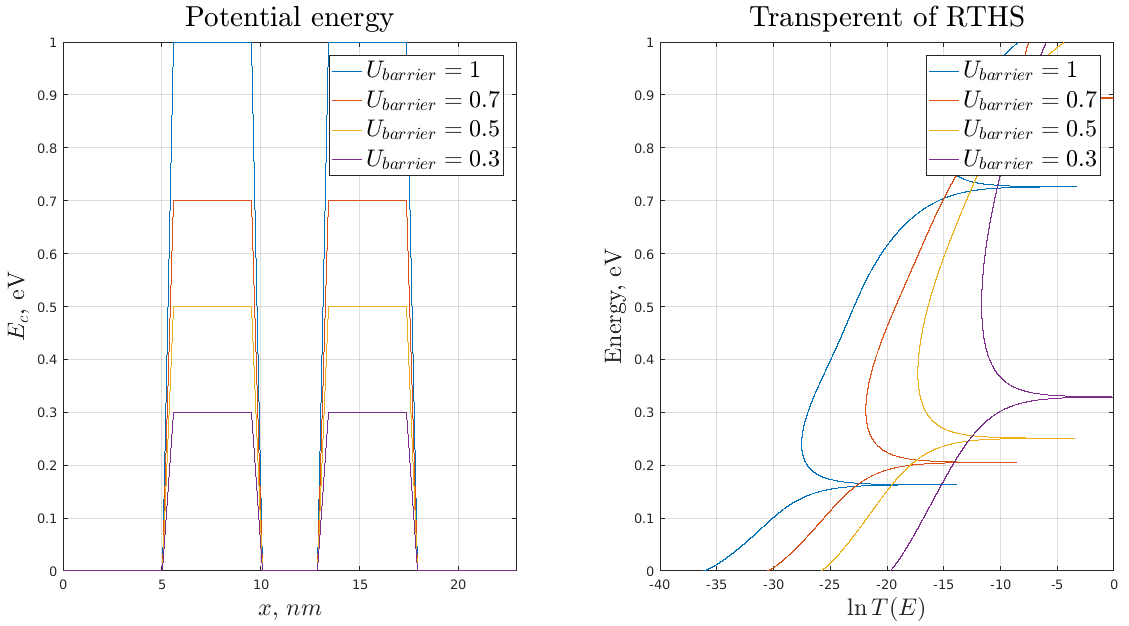
\includegraphics[width=.88\linewidth,center]{assets/qwt}\\
		{\color{red} Плотность тока через РТГС:}\\
	   	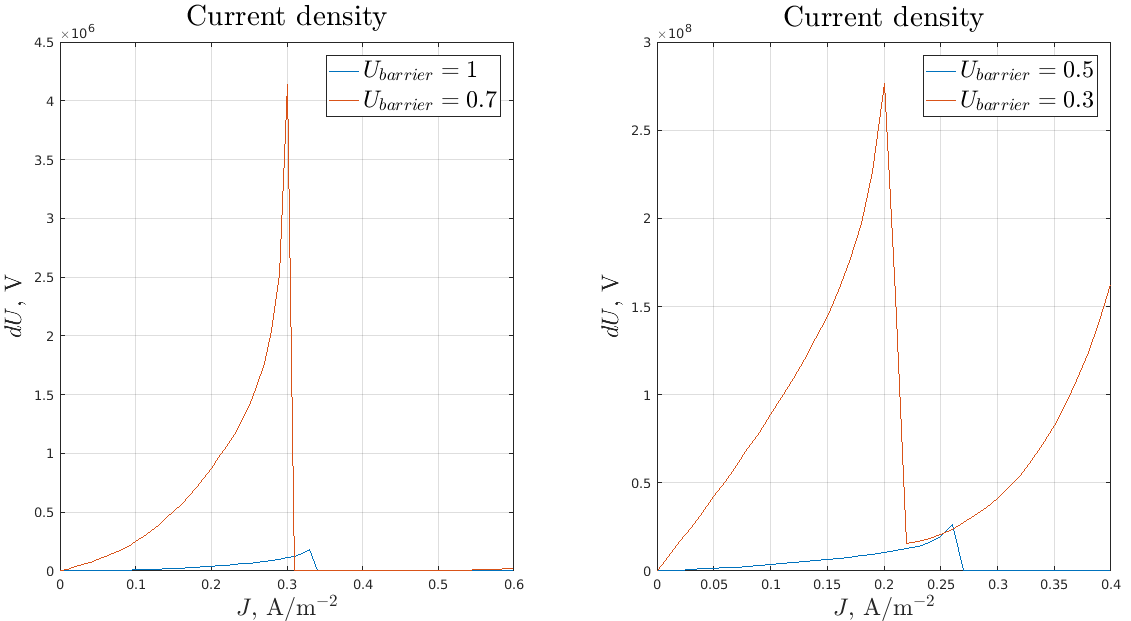
\includegraphics[width=.88\linewidth,center]{assets/qwj}
	\end{columns}
\end{frame}

\begin{frame}
	\frametitle{Исследование влияния параметров барьеров РТГС на ВАХ}
	\begin{columns}
	\column{0.5\textwidth}
		{\color{blue} Ширина барьеров:}\\
		{\color{red} Прозрачность РТГС:}
	   	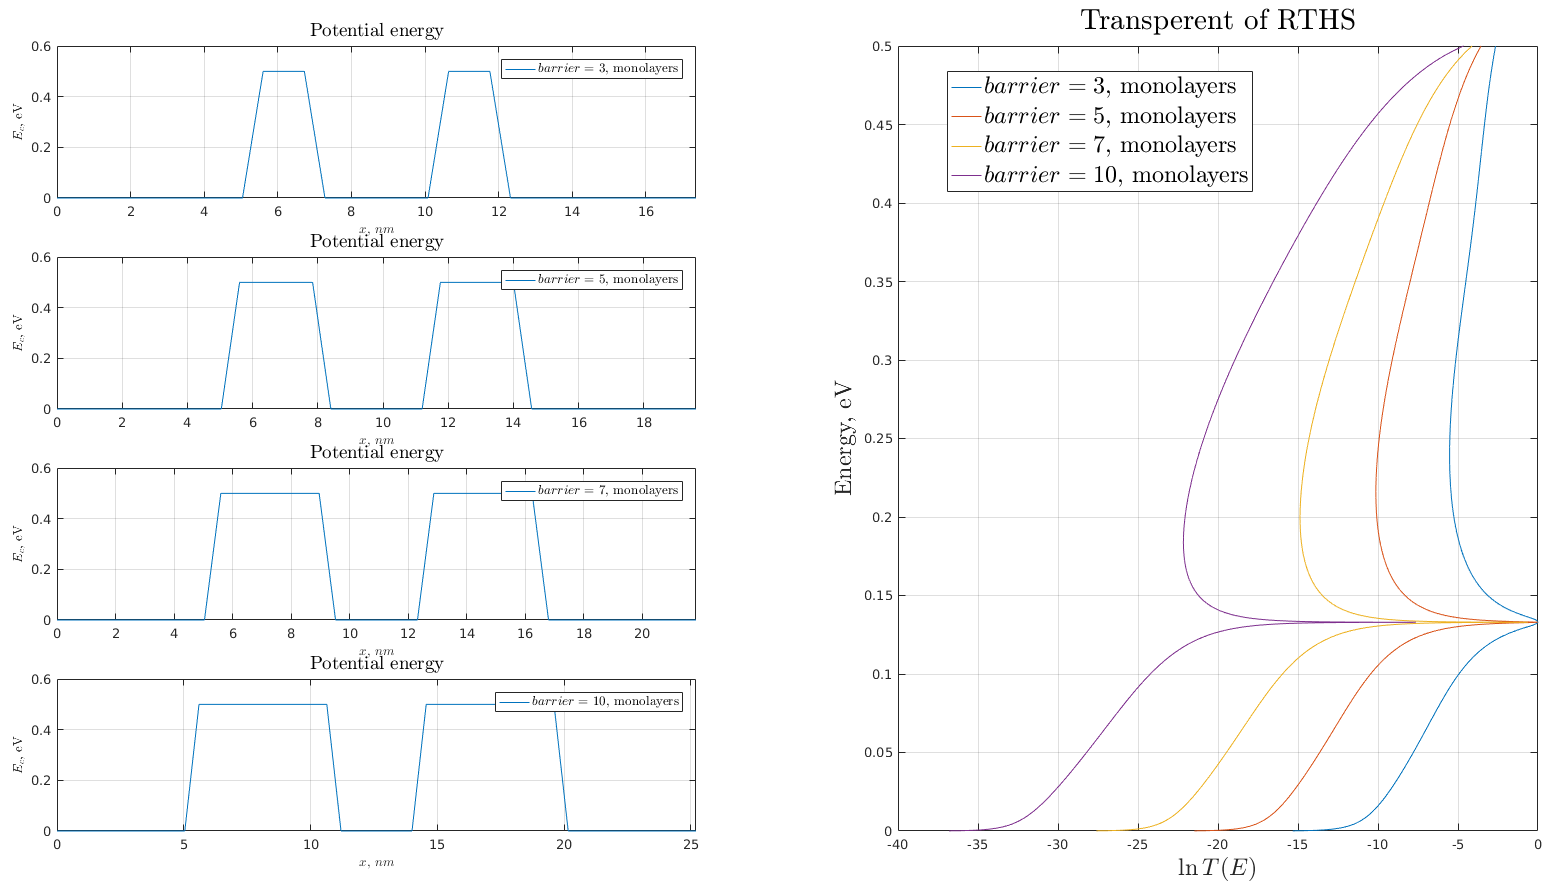
\includegraphics[width=.86\linewidth,center]{assets/qbwt}\\
		{\color{red} Плотность тока через РТГС:}
	   	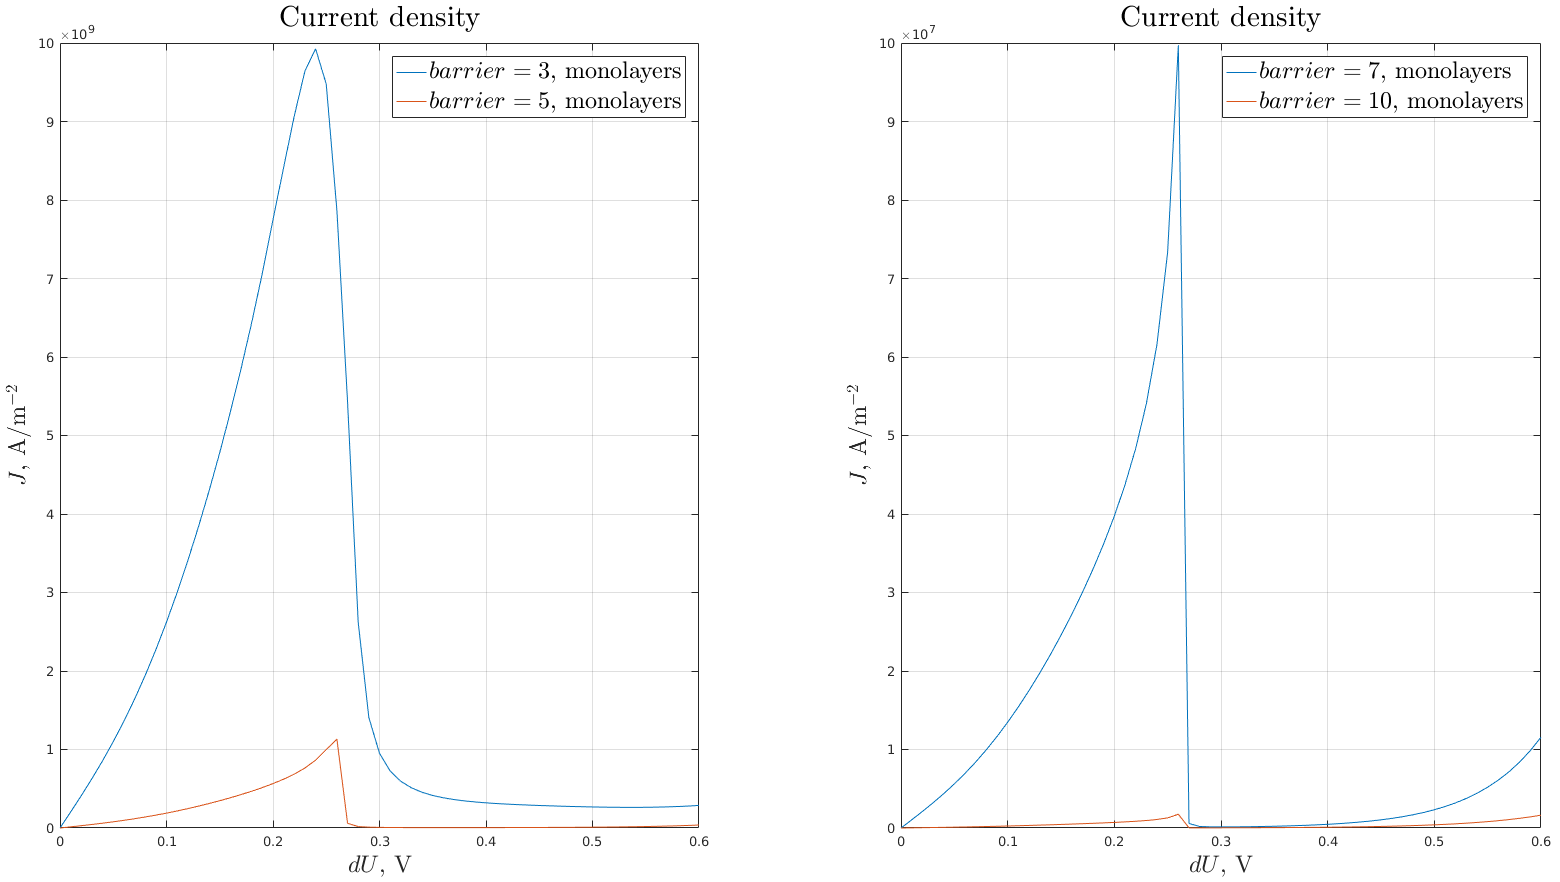
\includegraphics[width=.88\linewidth,center]{assets/qbwj}
	\column{0.01\textwidth}
		\rule[-55mm]{0.2ex}{75mm}
	\column{0.5\textwidth}
		{\color{blue} Высота барьеров:}\\
		{\color{red}\small Прозрачность РТГС:}\\
	   	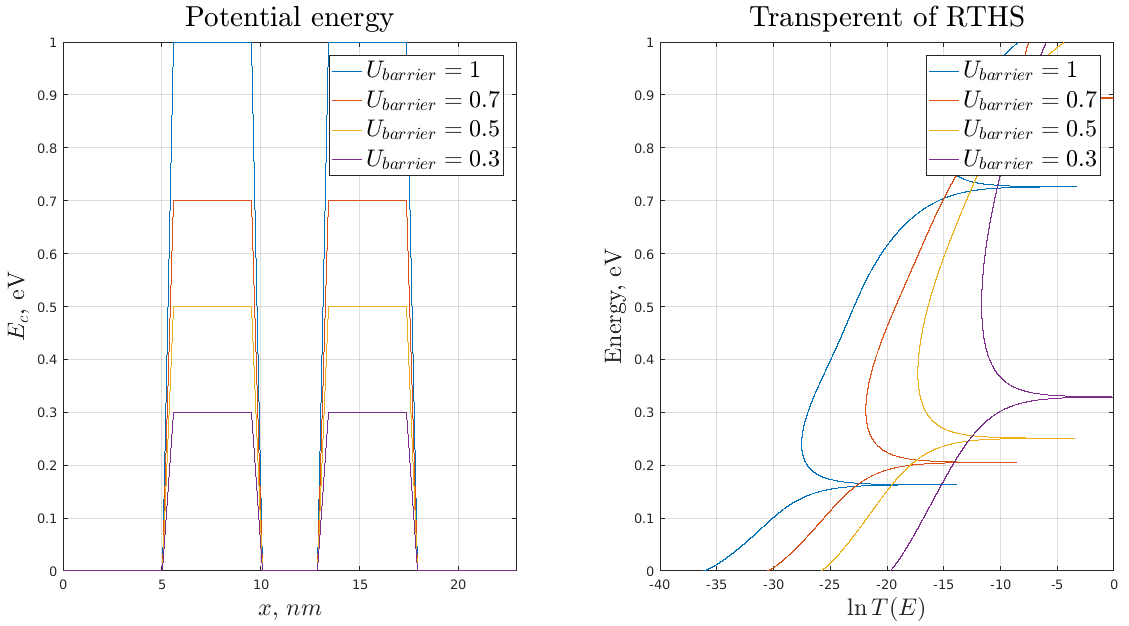
\includegraphics[width=.88\linewidth,center]{assets/qwt}\\
		{\color{red} Плотность тока через РТГС:}\\
	   	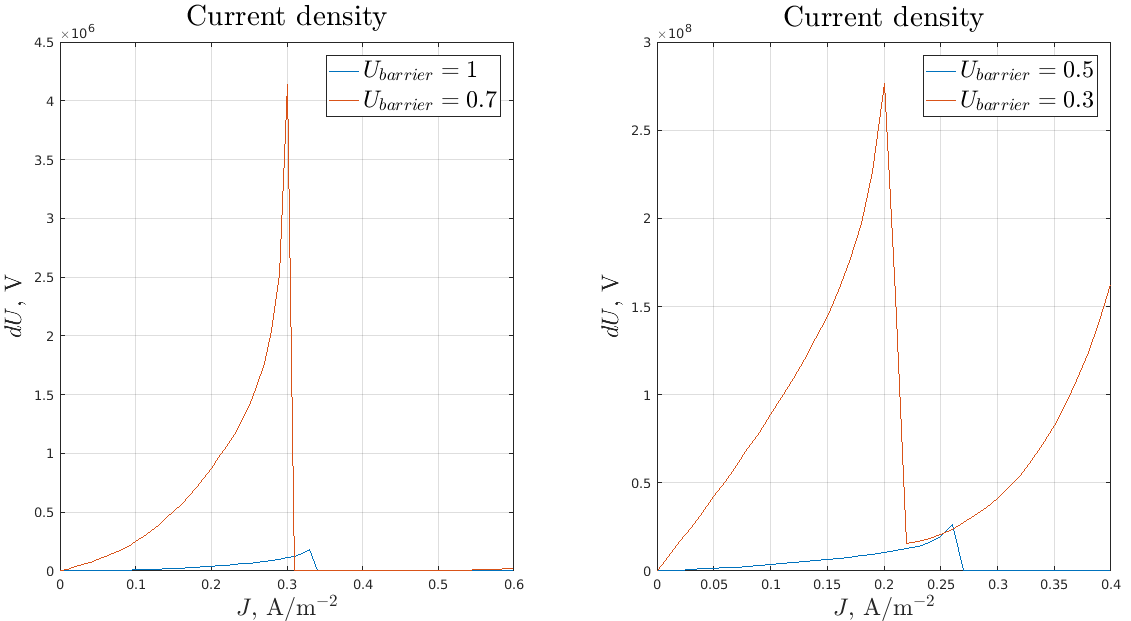
\includegraphics[width=.88\linewidth,center]{assets/qwj}
	\end{columns}
\end{frame}

\begin{frame}
	\frametitle{Исследование влияния параметров спейсера РТГС на ВАХ}
	\begin{columns}
	\column{0.5\textwidth}
		{\color{blue} Ширина спейсера:}\\
		{\color{red} Прозрачность РТГС:}
	   	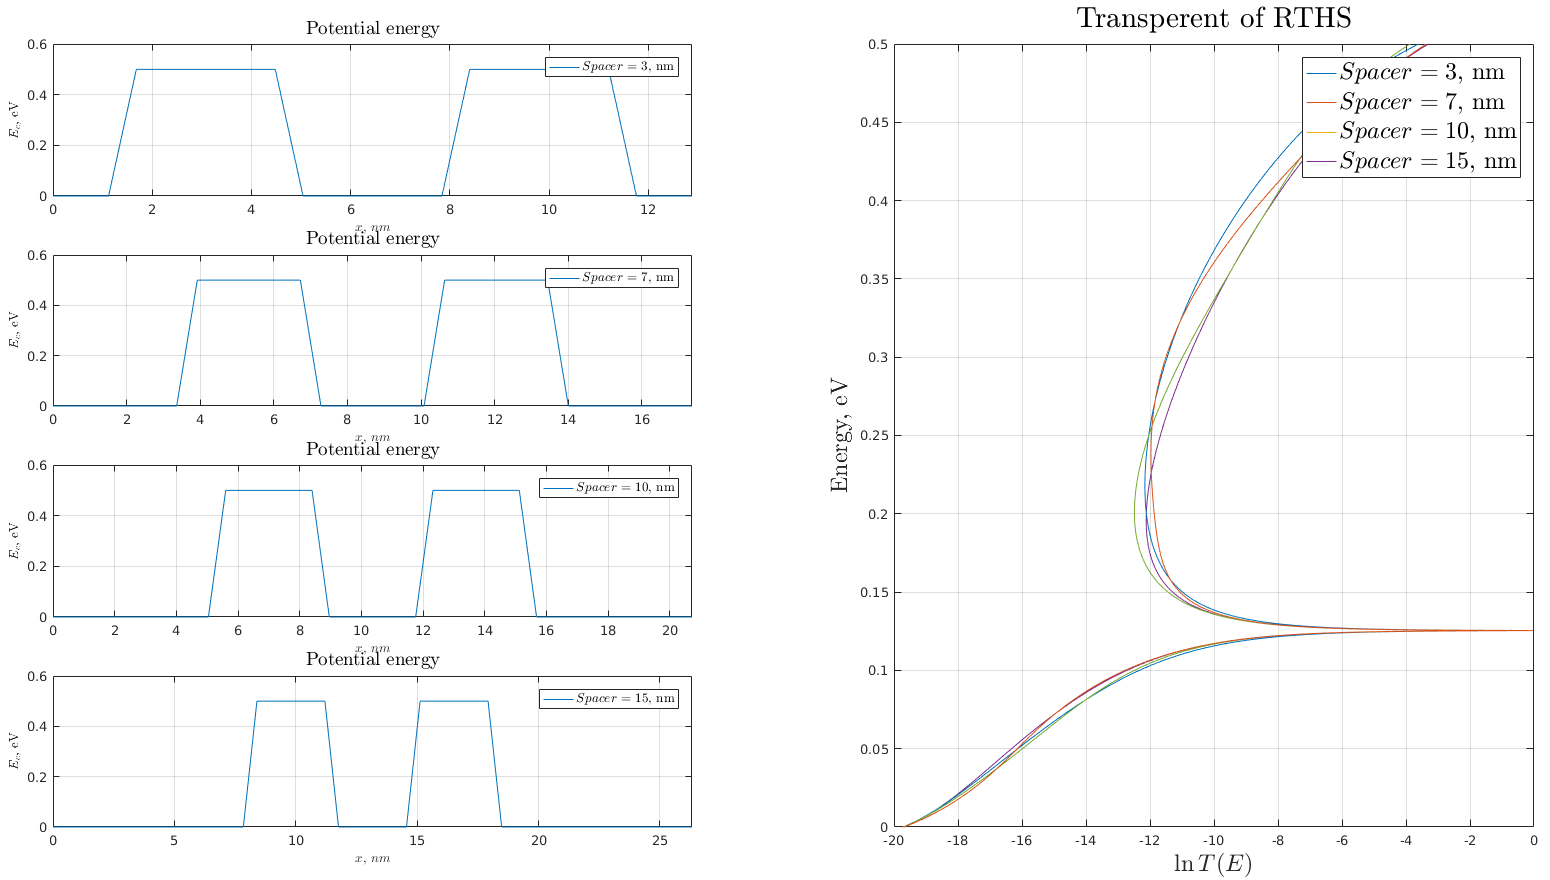
\includegraphics[width=.86\linewidth,center]{assets/qslt}\\
		{\color{red} Плотность тока через РТГС:}
	   	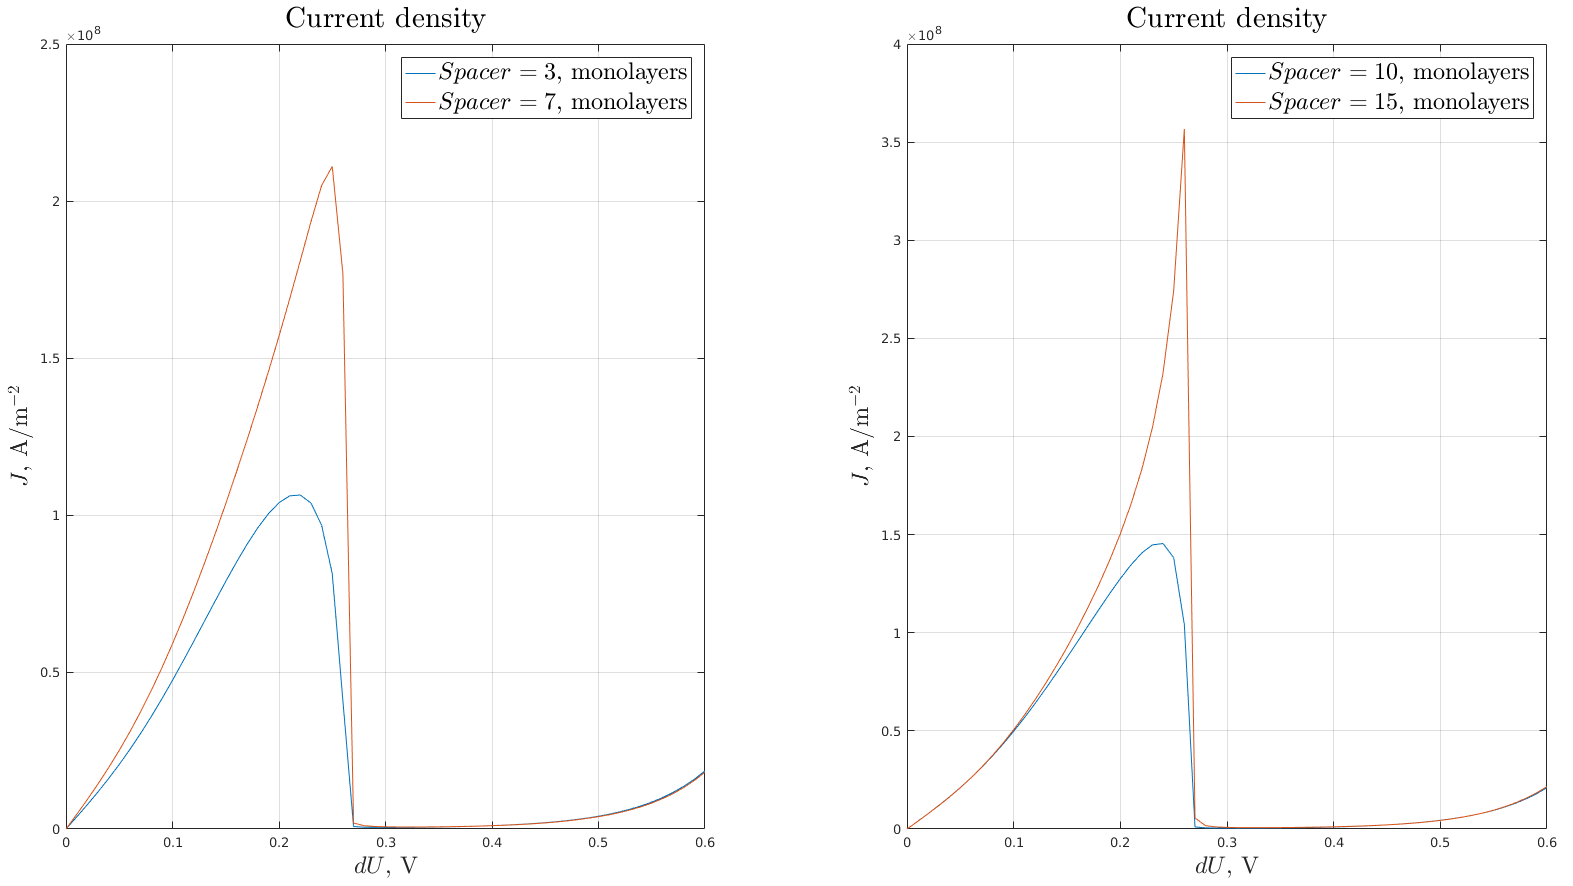
\includegraphics[width=.86\linewidth,center]{assets/qslj}
	\column{0.01\textwidth}
		\rule[-55mm]{0.2ex}{75mm}
	\column{0.5\textwidth}
		{\color{blue} Ширина спейсера с учетом ССП:}\\
		{\color{red} Плотность тока через РТГС:}
	   	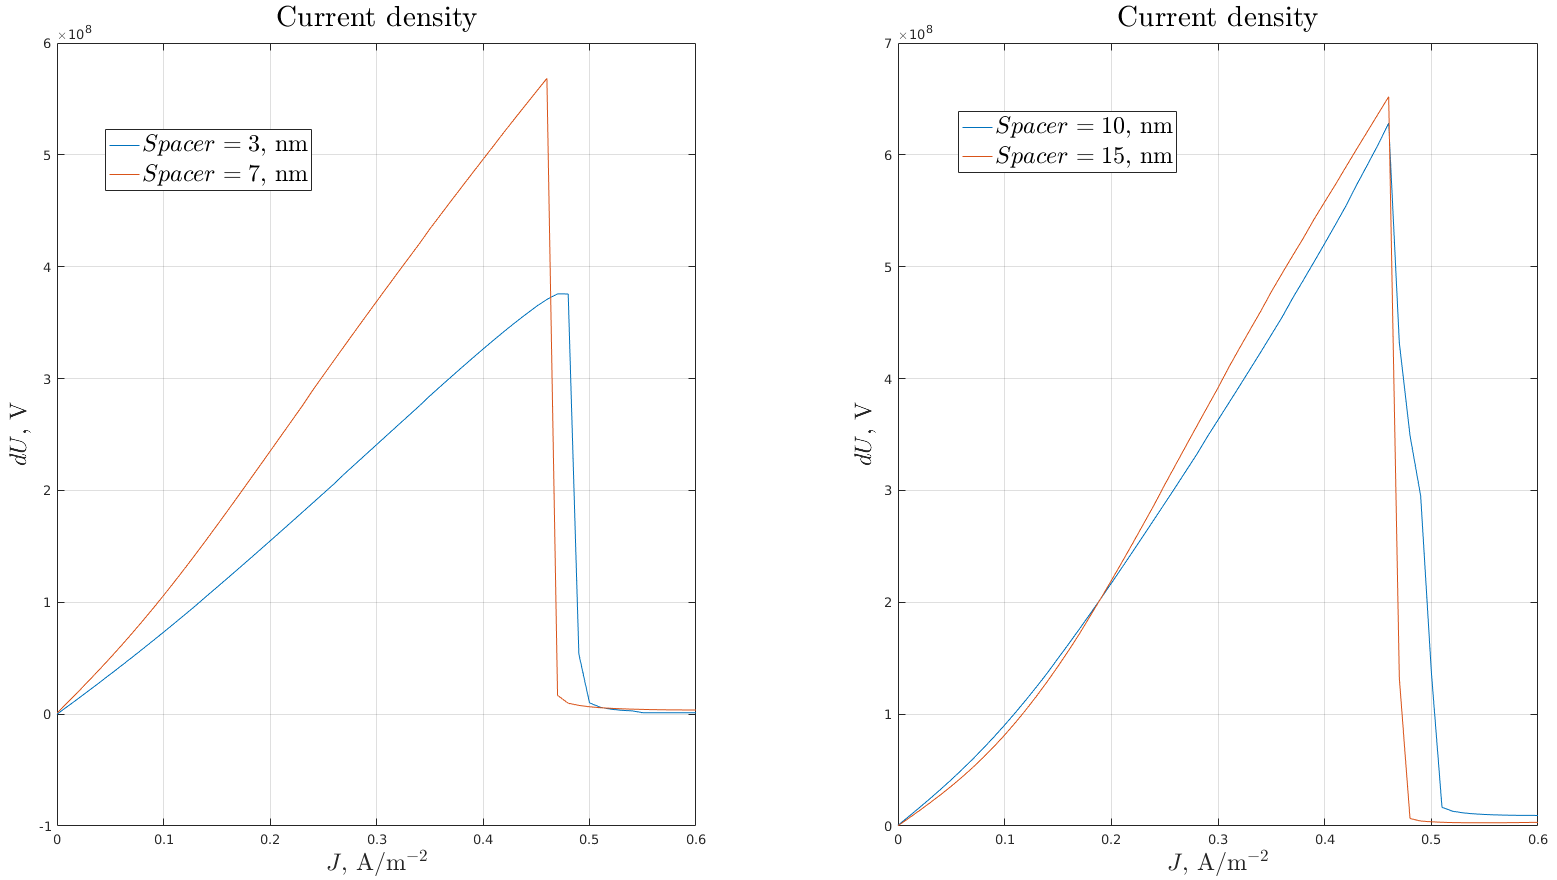
\includegraphics[width=.88\linewidth,center]{assets/qslqj}
	   	\\[39mm]
		{\color{red} }
	\end{columns}
\end{frame}

\begin{frame}
	\frametitle{Моделирование термической деградации ВАХ $Al_{x}Ga_{1-x}As$ РТГС}
	{\color{blue}\large Исследуемая модель:}
	\begin{columns}
	\column{0.6\textwidth}
		{\color{red} Схема:}
	   	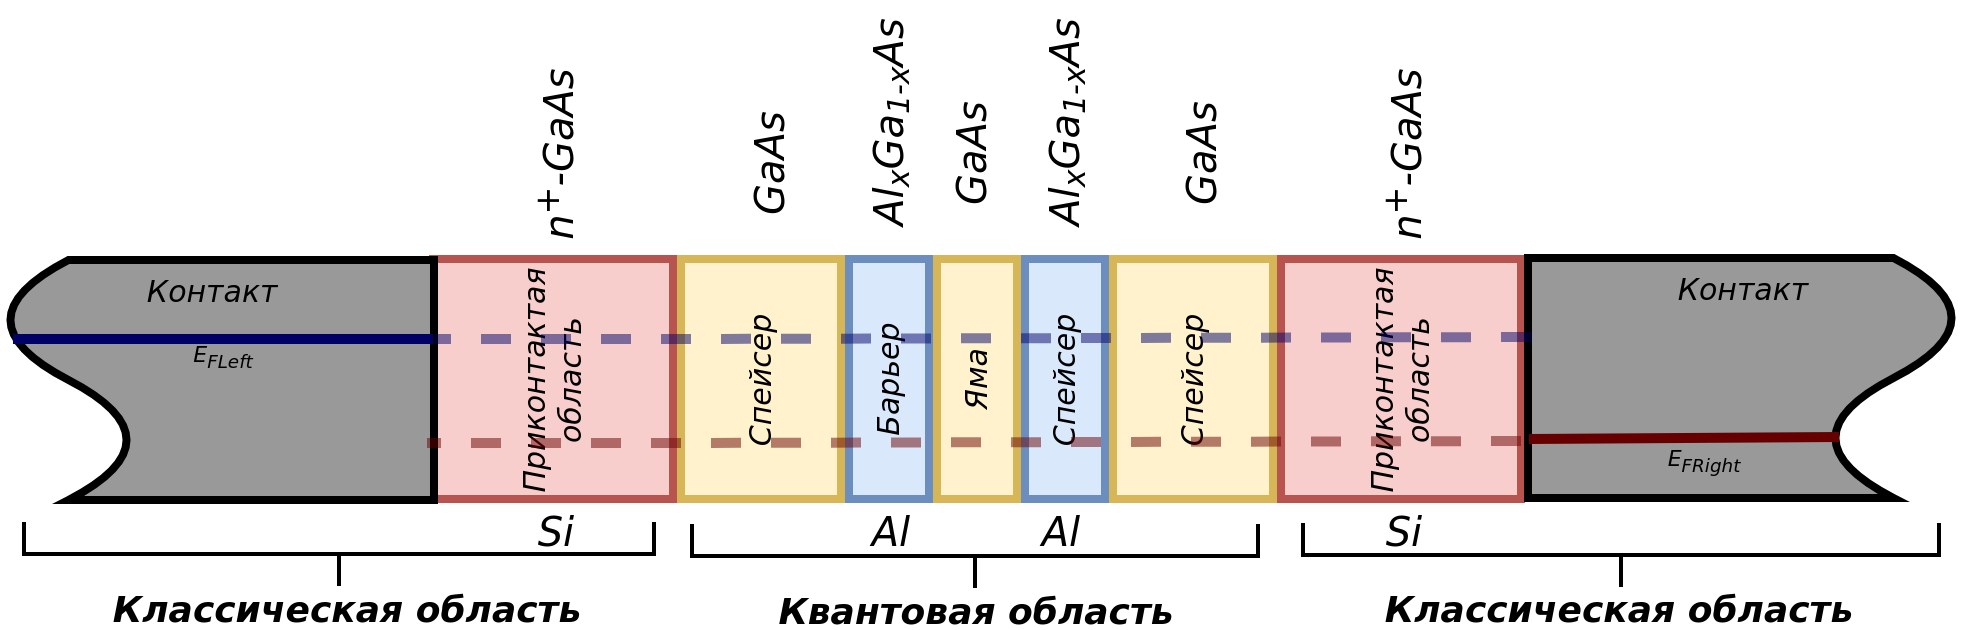
\includegraphics[width=.99\linewidth,center]{assets/RTHSModelDiff}
	\column{0.3\textwidth}
		{\color{red} Зонная структура:}
	   	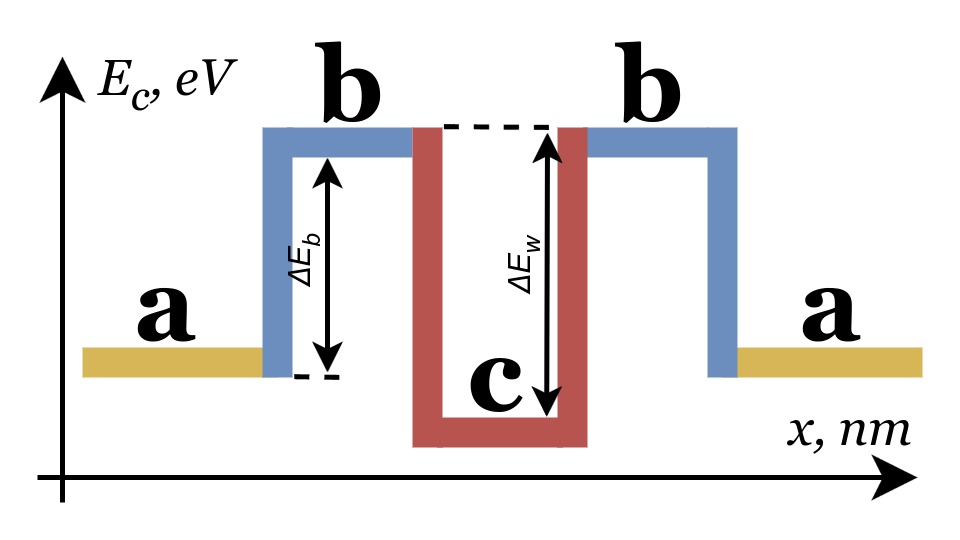
\includegraphics[width=.99\linewidth,center]{assets/BD}
	\end{columns}
{\color{red}Структура}: $n^{+}$-$GaAs$/$i$-$GaAs$/$i$-$Al_{0.4}Ga_{0.6}As$/$i$-$GaAs$/$i$-$Al_{0.4}Ga_{0.6}As$/$i$-$GaAs$/$n^{+}$-$GaAs$
	\begin{columns}
	\column{0.33\textwidth}
		{\color{blue} $Al_{x}Ga_{1-x}As$:}\\
		{\color{red}\footnotesize Период решетки:}\\
		\scriptsize
			$p = 0.56$ нм;\\
		{\color{red}\footnotesize Ширина запрященной зоны:}\\
		\scriptsize
			$p = 0.56$ нм;\\
		{\color{red}\footnotesize Эффективная масса в ЗП:}\\
		\scriptsize
			$p = 0.56$ нм;\\
		{\color{red}\footnotesize Число атомов:}\\
		\scriptsize
			$p = 0.56$ нм;\\
	\column{0.33\textwidth}
		{\color{blue} Параметры модели:}\\
		{\color{red}\footnotesize Размеры:}\\
		\scriptsize
			$p = 0.56$ монослоев;\\
			$p = 0.56$ монослоев;\\
			$p = 0.56$ монослоев;\\
		{\color{red}\footnotesize Зонная структура:}\\
			$\Delta E_{c} = \Delta E_{w} = 123x;$
	\column{0.33\textwidth}
		{\color{blue} Параметры диффузии:}
		\scriptsize
		\begin{equation*}
			D_{Al,Si} = D_{0}\exp\bigg[-\frac{E_{a}}{k_{B}T}\bigg]\Big( \frac{N_{D}}{n_{i}} \Big)^{3};
		\end{equation*}
		$E_{a} = 3.5$эВ -- энергия активации;\\
		$T = 360$K -- температура системы;\\
		$D_{0} = 0.2$ -- предъэксподенциальный множитель;\\
		$N_{D}$ -- концентрация донорной примеси;\\
		$n_{i}$ -- концентрация собственных носителей заряда.
	\end{columns}
\end{frame}

\begin{frame}
	\frametitle{Моделирование термической деградации квантовой области}
	\centering
	% {\color{blue}$GaAs$/$Al_{0.4}Ga_{0.6}As$/$GaAs$/$Al_{0.4}Ga_{0.6}As$/$GaAs$}
	\begin{columns}
	\column{0.5\textwidth}
		{\color{blue} $N_{D} = n_{i} = 10^{12} m^{-3},\,T = 800K$:}\\
		{\color{red} Диффузионное расплытие профиля:}\\
	   	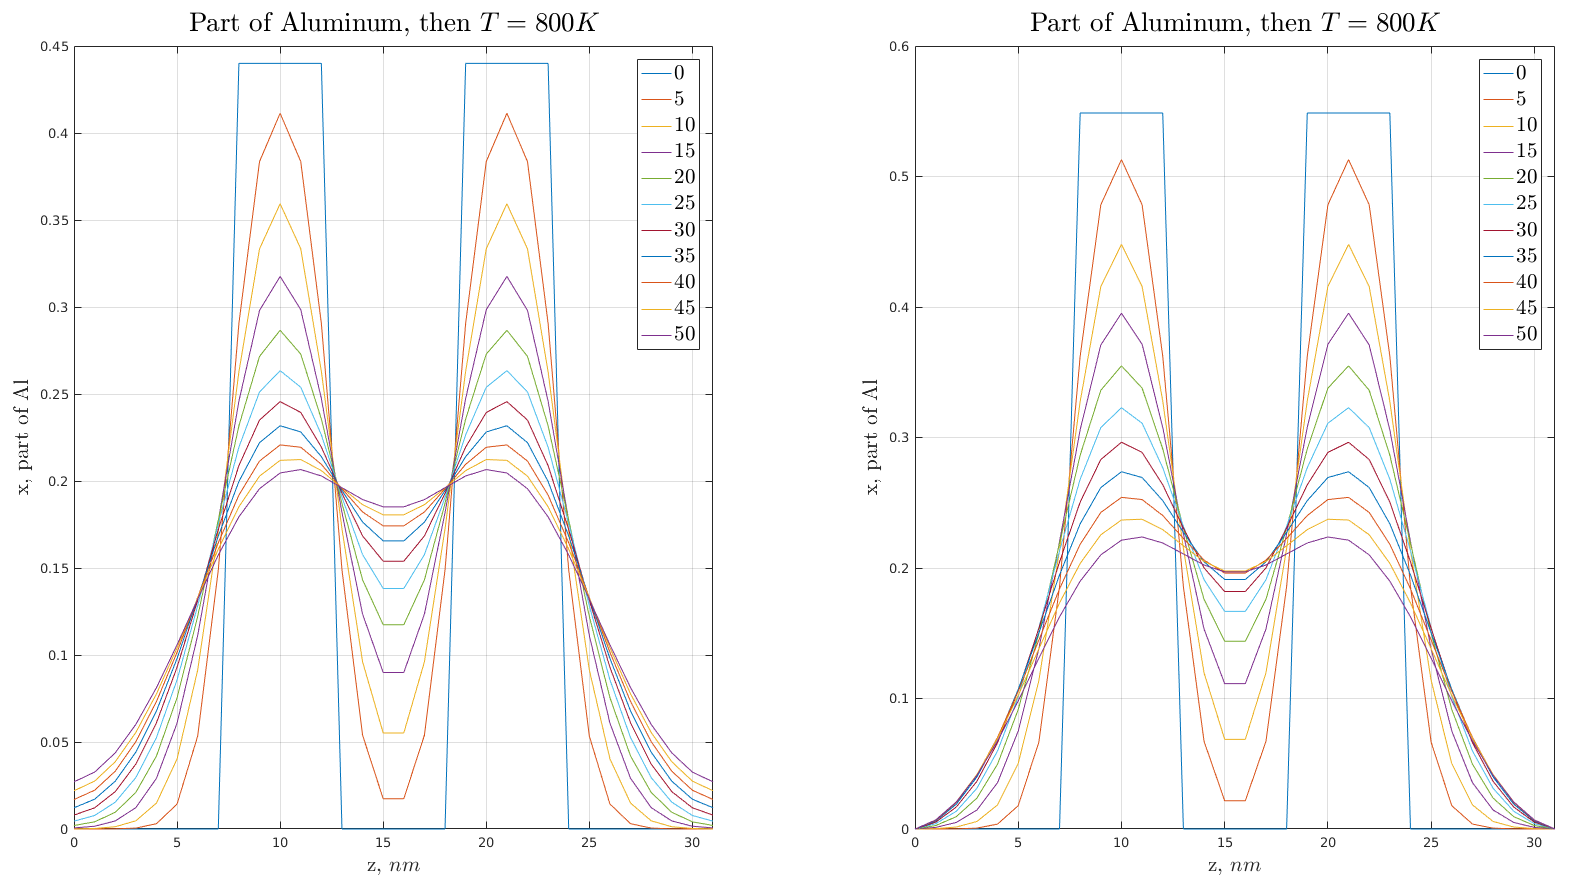
\includegraphics[width=0.85\linewidth,center]{assets/DCAlGaAs}\\
		{\color{red} Деградация ВАХ:}
	   	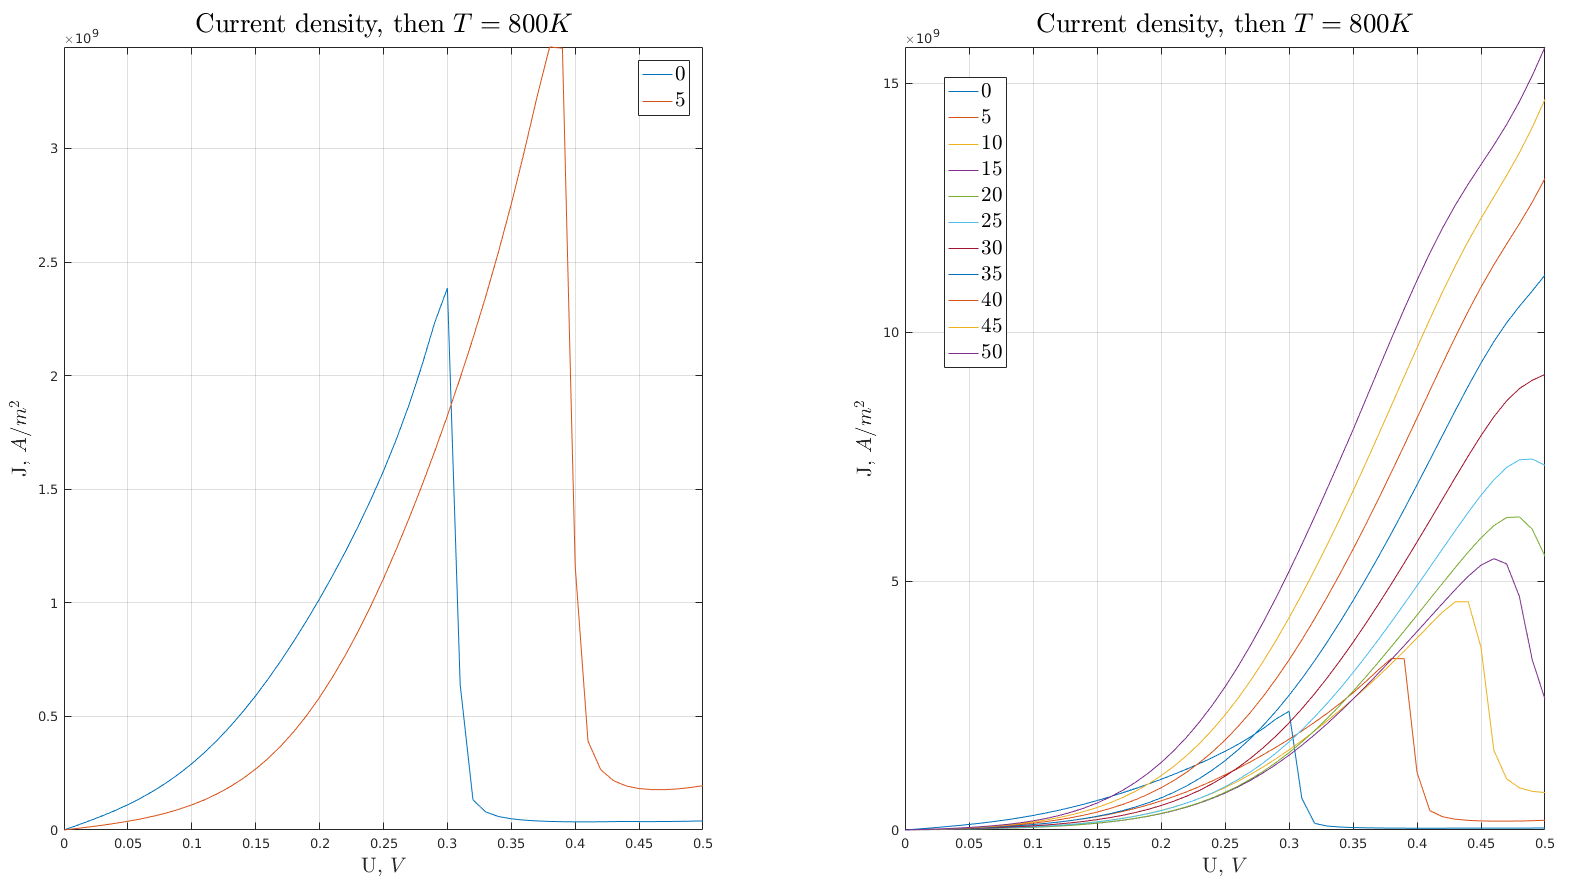
\includegraphics[width=.9\linewidth,center]{assets/JDCAlGaAs}
	   	\newline\newline\newline\newline
	\column{0.01\textwidth}
		\rule[17mm]{0.2ex}{76mm}
	\column{0.5\textwidth}
		{\color{blue} $N_{D} = 10^{18}; n_{i} = 10^{12} m^{-3};\,T = 650K$:}
		{\color{red} Диффузионное расплытие профиля:}\\
	   	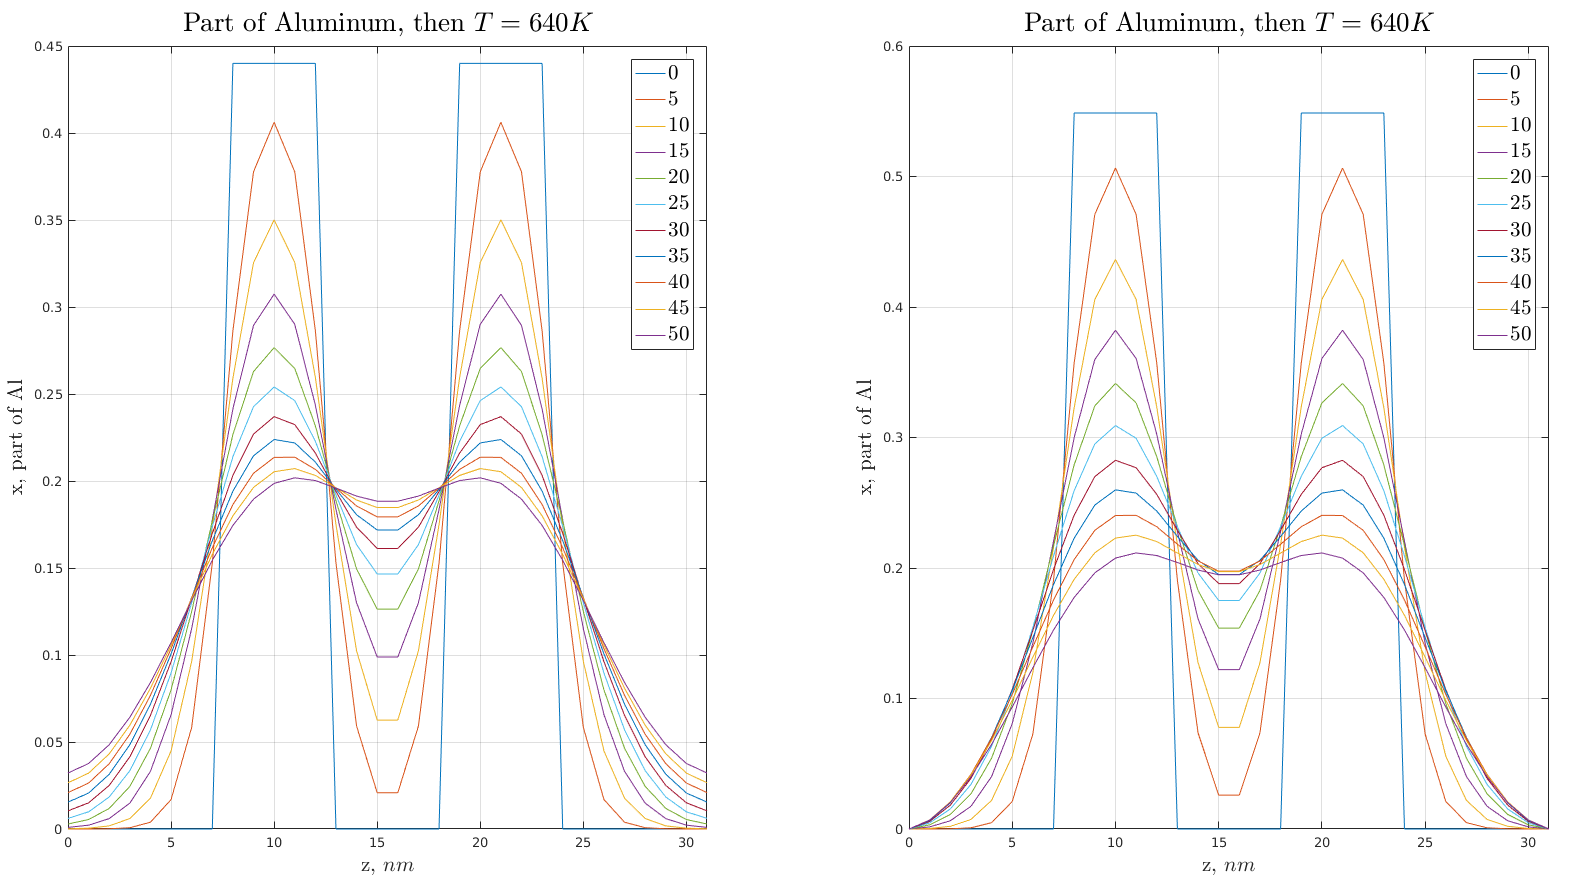
\includegraphics[width=.85\linewidth,center]{assets/DCAlGaAsNd}\\
		{\color{red} Деградация ВАХ:}\\
	   	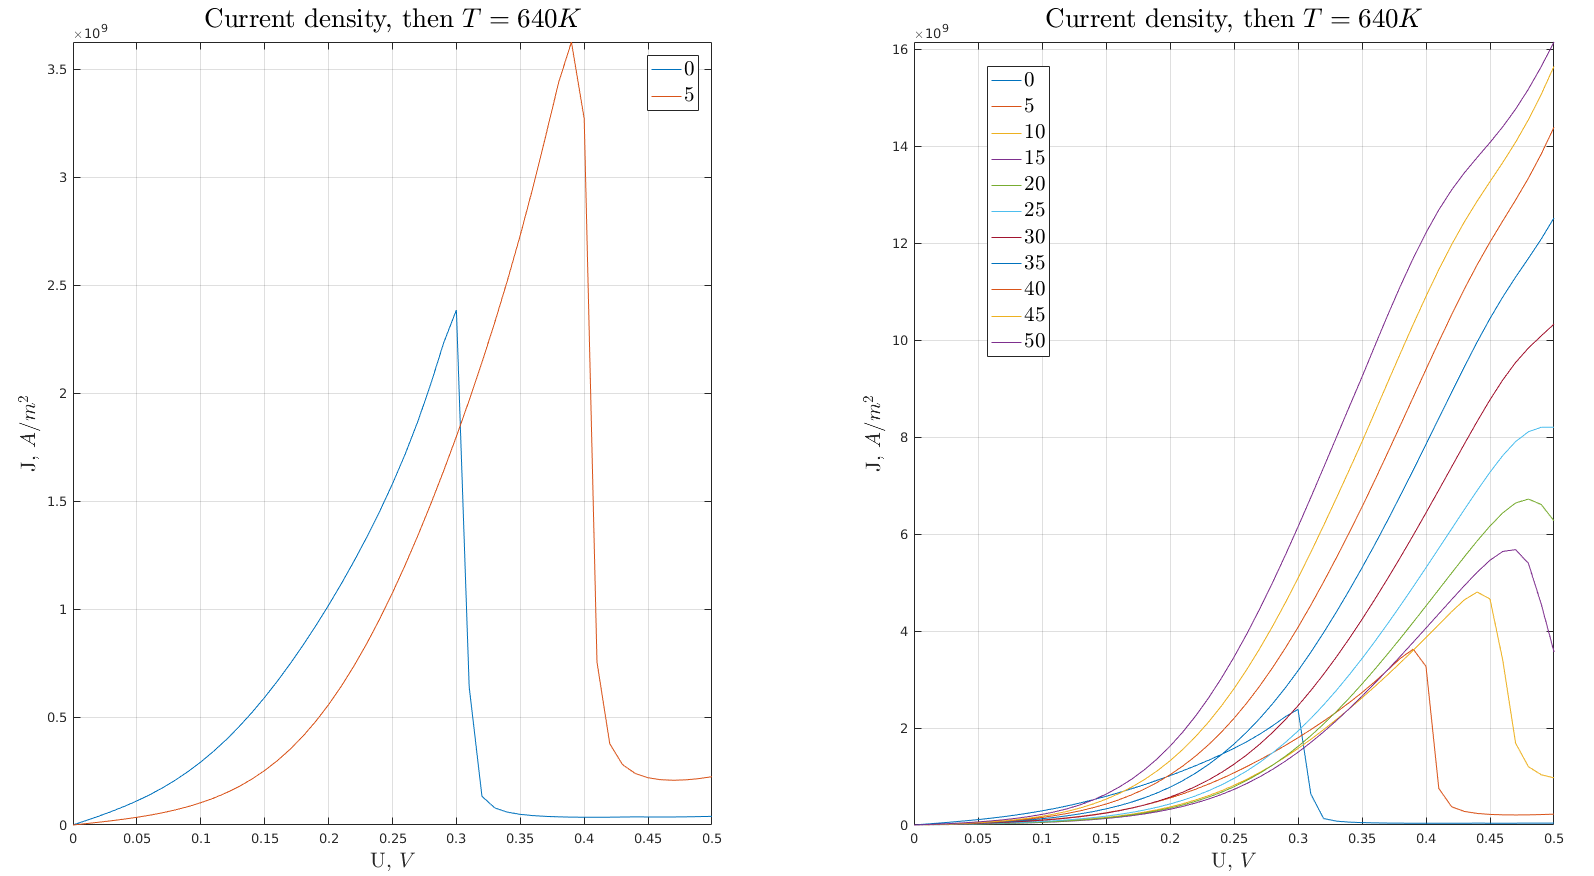
\includegraphics[width=.9\linewidth,center]{assets/JDCAlGaAsNd}
	   	\newline\newline\newline\newline
	\end{columns}
\end{frame}

\begin{frame}
	\frametitle{Моделирование термической деградации квантовой области с учетом приконтактных областей}
	{\large\color{blue} $N_{D}^{Reserve} = 10^{24}m^{-3};\,N_{D} = n_{i} = 10^{12} m^{-3},\,T = 800K$:}\\
	\begin{columns}
	\column{0.5\textwidth}
		{\color{red} Диффузионное расплытие профиля:}\\
	   	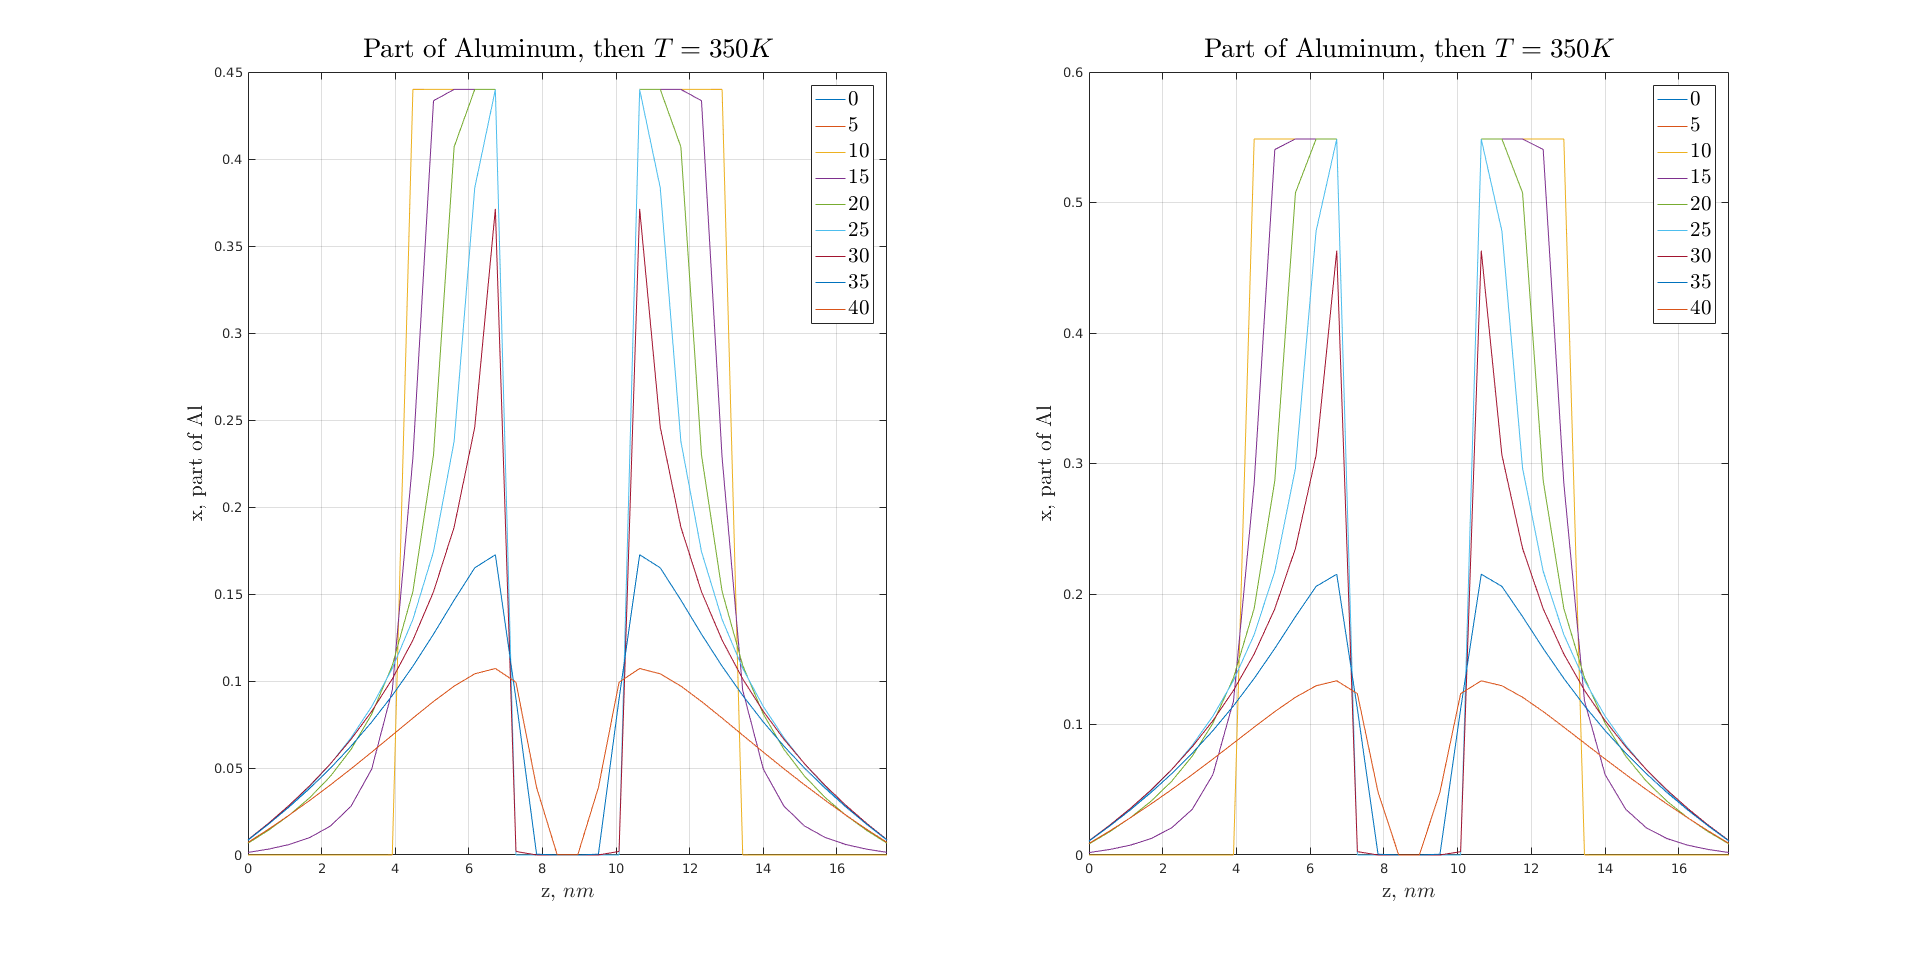
\includegraphics[width=.99\linewidth,center]{assets/DAlGaAs_Si}\\
	\column{0.01\textwidth}
		\rule[0mm]{0.2ex}{40mm}
	\column{0.5\textwidth}
		{\color{red} Деградация ВАХ:}\\
	   	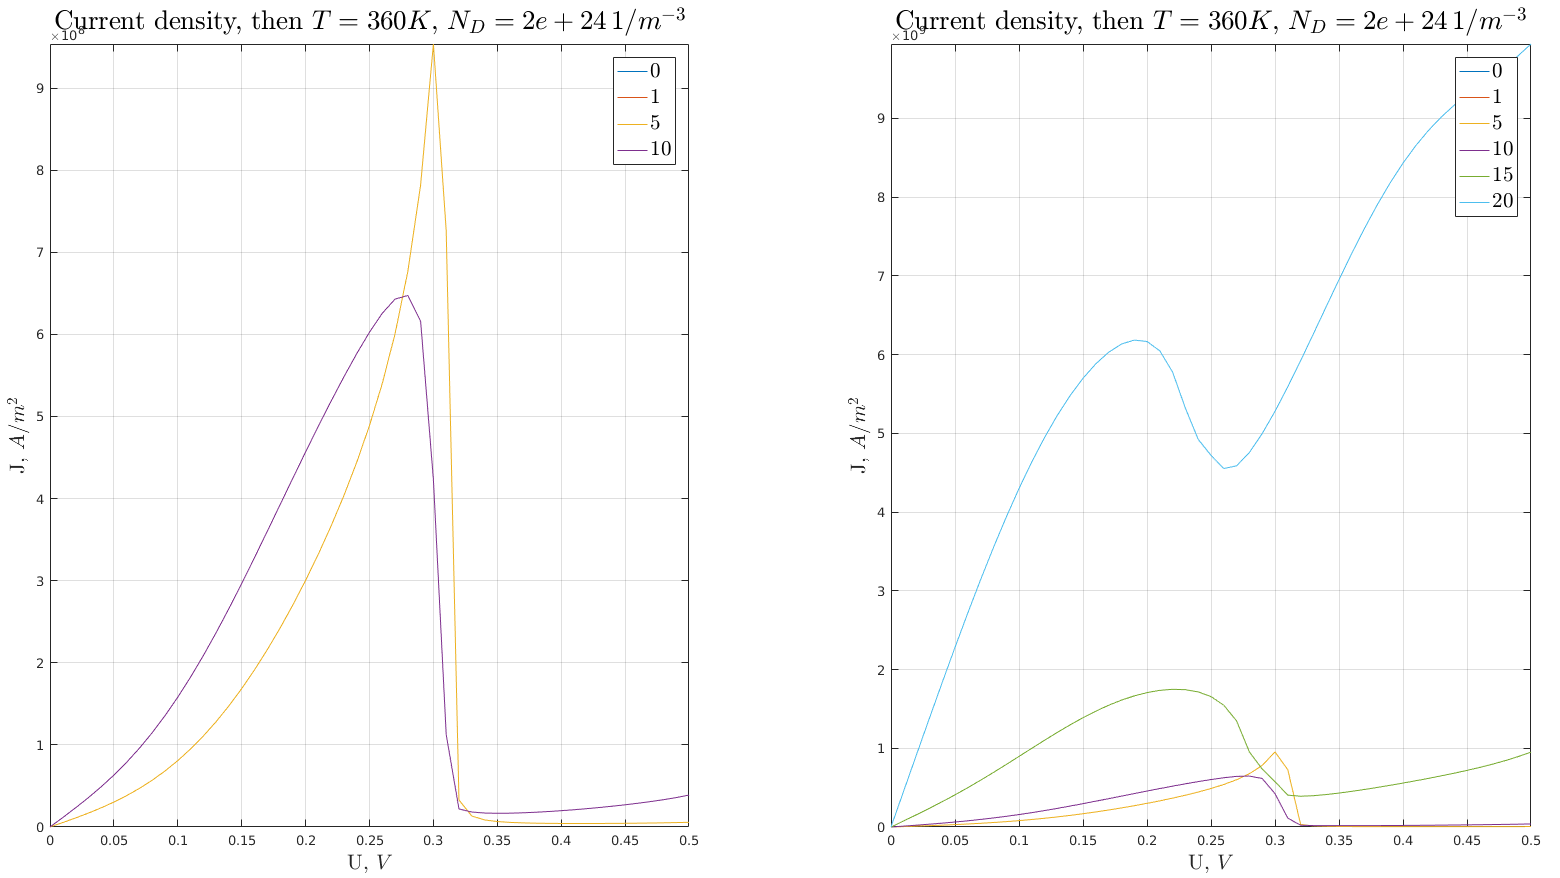
\includegraphics[width=.99\linewidth,center]{assets/JDAlGaAs_Si}\\
	\end{columns}
	{\large\color{blue}Вывод:}\\
\end{frame}

\begin{frame}
	\frametitle{Заключение}
\end{frame}

\begin{frame}
	\frametitle{Спасибо за внимание!}
\end{frame}

\end{document}


% \begin{frame}
% 	\frametitle{Цели и задачи}
% \end{frame}

% \begin{columns}
% \column{0.5\textwidth}
% \column{0.5\textwidth}
% \end{columns}

% \rule[4mm]{0.2ex}{60mm}